\documentclass[11pt]{article}
\usepackage[utf8]{inputenc}
\usepackage[T1]{fontenc}
\usepackage{textcomp}
\usepackage[a4paper,margin=2.1cm]{geometry}
\usepackage{amsmath,amssymb}
\usepackage{tikz}
\usepackage{xcolor}
\usepackage{mdframed}
\usepackage{enumitem}
\usepackage[colorlinks=true,linkcolor=blue!60!black]{hyperref}
\setlength{\parindent}{0pt}
\setlength{\parskip}{6pt}

\newcommand{\question}[1]{\par\medskip\noindent\textbf{#1}\par}
\newmdenv[linecolor=green!45!black,linewidth=0.8pt,backgroundcolor=green!4,
  innertopmargin=4pt,innerbottommargin=4pt,skipabove=6pt,skipbelow=6pt]{answerbox}

\title{\textbf{Expanding Brackets}\\[0.3em]\large Worked Solutions with Area-Model Diagrams}
\author{Wisest Maths --- Year 1 A-Level, Algebra (ref \texttt{a1})}
\date{}

\begin{document}
\maketitle
\noindent This document contains all 45 \emph{Expanding Brackets} questions, each with a fully worked
solution and a TikZ \emph{area-model} (box-method) diagram. In an area model the terms of one
bracket label the rows, the terms of the other label the columns, and each interior cell holds the
product of its row and column headings; summing the cells (and collecting like terms) gives the
expansion.
\tableofcontents
\bigskip
\hrule

\section*{Expanding Brackets 01\quad\small\texttt{(a1-001)}}
\addcontentsline{toc}{section}{Expanding Brackets 01 (a1-001)}
\textit{Difficulty: Foundation \quad\textbar\quad Marks: 2}

\question{Expand the brackets \((x+4)(x-1)\).}

\textbf{Worked solution.}

\textit{Expand and simplify}
\[\begin{gathered}
\text{Expanding the brackets:} \\[1em] \begin{aligned} (x+4)(x-1) &= x(x-1)+4(x-1) \\ &= x^2-x+4x-4 \\ &= x^2+3x-4 \end{aligned}
\end{gathered}\]
Multiply each term in the first bracket by each term in the second, then collect like terms.

\begin{answerbox}
\textbf{Final answer:}\quad \(\displaystyle x^2+3x-4\)
\end{answerbox}
\textbf{Common mistake.} A common mistake is to forget to multiply the \(4\) by the \(-1\), which gives the incorrect answer \(x^2+3x+4\).

\textbf{Area-model diagram.}

\begin{center}
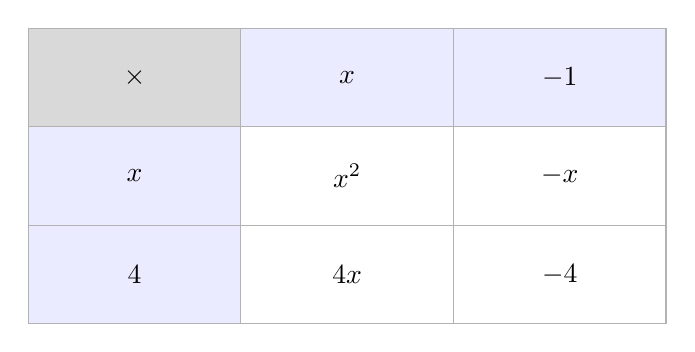
\begin{tikzpicture}[x=1cm,y=1cm]
\fill[gray!30] (0,0) rectangle (2.7,-1.25);
\draw[gray!60] (0,0) rectangle (2.7,-1.25);
\node at (1.35,-0.625) {$\displaystyle \times$};
\fill[blue!8] (2.7,0) rectangle (5.4,-1.25);
\draw[gray!60] (2.7,0) rectangle (5.4,-1.25);
\node at (4.05,-0.625) {$\displaystyle x$};
\fill[blue!8] (5.4,0) rectangle (8.1,-1.25);
\draw[gray!60] (5.4,0) rectangle (8.1,-1.25);
\node at (6.75,-0.625) {$\displaystyle -1$};
\fill[blue!8] (0,-1.25) rectangle (2.7,-2.5);
\draw[gray!60] (0,-1.25) rectangle (2.7,-2.5);
\node at (1.35,-1.875) {$\displaystyle x$};
\fill[white] (2.7,-1.25) rectangle (5.4,-2.5);
\draw[gray!60] (2.7,-1.25) rectangle (5.4,-2.5);
\node at (4.05,-1.875) {$\displaystyle x^2$};
\fill[white] (5.4,-1.25) rectangle (8.1,-2.5);
\draw[gray!60] (5.4,-1.25) rectangle (8.1,-2.5);
\node at (6.75,-1.875) {$\displaystyle -x$};
\fill[blue!8] (0,-2.5) rectangle (2.7,-3.75);
\draw[gray!60] (0,-2.5) rectangle (2.7,-3.75);
\node at (1.35,-3.125) {$\displaystyle 4$};
\fill[white] (2.7,-2.5) rectangle (5.4,-3.75);
\draw[gray!60] (2.7,-2.5) rectangle (5.4,-3.75);
\node at (4.05,-3.125) {$\displaystyle 4x$};
\fill[white] (5.4,-2.5) rectangle (8.1,-3.75);
\draw[gray!60] (5.4,-2.5) rectangle (8.1,-3.75);
\node at (6.75,-3.125) {$\displaystyle -4$};
\end{tikzpicture}
\end{center}
\medskip\hrule

\section*{Expanding Brackets 02\quad\small\texttt{(a1-002)}}
\addcontentsline{toc}{section}{Expanding Brackets 02 (a1-002)}
\textit{Difficulty: Foundation \quad\textbar\quad Marks: 2}

\question{Expand the brackets \((2x+1)(x-3)\).}

\textbf{Worked solution.}

\textit{Expand and simplify}
\[\begin{gathered}
\text{Expanding the brackets:} \\[1em] \begin{aligned} (2x+1)(x-3) &= 2x(x-3)+1(x-3) \\ &= 2x^2-6x+x-3 \\ &= 2x^2-5x-3 \end{aligned}
\end{gathered}\]
Multiply each term in the first bracket by each term in the second, then collect like terms.

\begin{answerbox}
\textbf{Final answer:}\quad \(\displaystyle 2x^2-5x-3\)
\end{answerbox}
\textbf{Common mistake.} A common mistake is to forget to multiply the \(-3\) by the \(1\), which gives the incorrect answer \(2x^2-6x-3\).

\textbf{Area-model diagram.}

\begin{center}
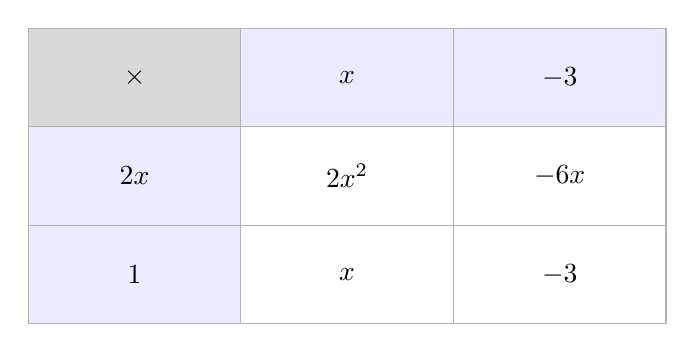
\begin{tikzpicture}[x=1cm,y=1cm]
\fill[gray!30] (0,0) rectangle (2.7,-1.25);
\draw[gray!60] (0,0) rectangle (2.7,-1.25);
\node at (1.35,-0.625) {$\displaystyle \times$};
\fill[blue!8] (2.7,0) rectangle (5.4,-1.25);
\draw[gray!60] (2.7,0) rectangle (5.4,-1.25);
\node at (4.05,-0.625) {$\displaystyle x$};
\fill[blue!8] (5.4,0) rectangle (8.1,-1.25);
\draw[gray!60] (5.4,0) rectangle (8.1,-1.25);
\node at (6.75,-0.625) {$\displaystyle -3$};
\fill[blue!8] (0,-1.25) rectangle (2.7,-2.5);
\draw[gray!60] (0,-1.25) rectangle (2.7,-2.5);
\node at (1.35,-1.875) {$\displaystyle 2x$};
\fill[white] (2.7,-1.25) rectangle (5.4,-2.5);
\draw[gray!60] (2.7,-1.25) rectangle (5.4,-2.5);
\node at (4.05,-1.875) {$\displaystyle 2x^2$};
\fill[white] (5.4,-1.25) rectangle (8.1,-2.5);
\draw[gray!60] (5.4,-1.25) rectangle (8.1,-2.5);
\node at (6.75,-1.875) {$\displaystyle -6x$};
\fill[blue!8] (0,-2.5) rectangle (2.7,-3.75);
\draw[gray!60] (0,-2.5) rectangle (2.7,-3.75);
\node at (1.35,-3.125) {$\displaystyle 1$};
\fill[white] (2.7,-2.5) rectangle (5.4,-3.75);
\draw[gray!60] (2.7,-2.5) rectangle (5.4,-3.75);
\node at (4.05,-3.125) {$\displaystyle x$};
\fill[white] (5.4,-2.5) rectangle (8.1,-3.75);
\draw[gray!60] (5.4,-2.5) rectangle (8.1,-3.75);
\node at (6.75,-3.125) {$\displaystyle -3$};
\end{tikzpicture}
\end{center}
\medskip\hrule

\section*{Expanding Brackets 03\quad\small\texttt{(a1-003)}}
\addcontentsline{toc}{section}{Expanding Brackets 03 (a1-003)}
\textit{Difficulty: Foundation \quad\textbar\quad Marks: 2}

\question{Expand the brackets \((x+1)(x-2)(x+3)\).}

\textbf{Worked solution.}

\textit{Expand the last two brackets first, then multiply by the remaining bracket}
\[\begin{gathered}
\text{Expanding the last two brackets:} \\[1em] \begin{aligned} (x+1)\Big((x-2)(x+3)\Big) &= (x+1)\Big(x^2+3x-2x-6\Big) \\ &= (x+1)\Big(x^2+x-6\Big) \end{aligned} \\[1em] \text{Now expand:} \\[1em] \begin{aligned} (x+1)\Big( x^2+x-6\Big)&= x(x^2+x-6)+1(x^2+x-6) \\ &= x^3+x^2-6x+x^2+x-6 \\ &= x^3+2x^2-5x-6 \end{aligned}
\end{gathered}\]
First expand two of the three brackets, then multiply the result by the third bracket.

\begin{answerbox}
\textbf{Final answer:}\quad \(\displaystyle x^3+2x^2-5x-6\)
\end{answerbox}
\textbf{Area-model diagram.}

\begin{center}
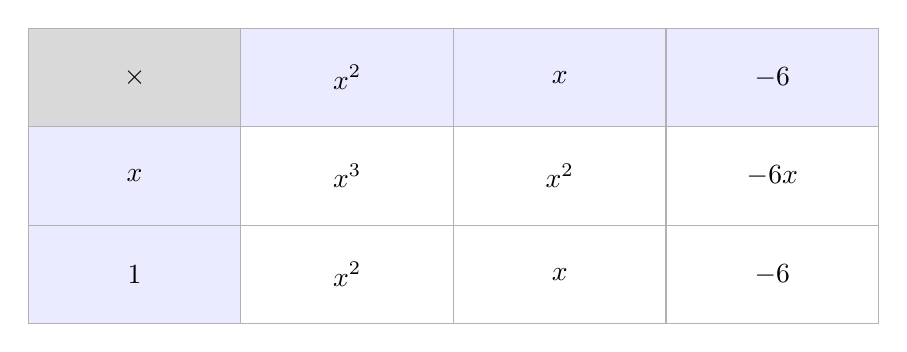
\begin{tikzpicture}[x=1cm,y=1cm]
\fill[gray!30] (0,0) rectangle (2.7,-1.25);
\draw[gray!60] (0,0) rectangle (2.7,-1.25);
\node at (1.35,-0.625) {$\displaystyle \times$};
\fill[blue!8] (2.7,0) rectangle (5.4,-1.25);
\draw[gray!60] (2.7,0) rectangle (5.4,-1.25);
\node at (4.05,-0.625) {$\displaystyle x^2$};
\fill[blue!8] (5.4,0) rectangle (8.1,-1.25);
\draw[gray!60] (5.4,0) rectangle (8.1,-1.25);
\node at (6.75,-0.625) {$\displaystyle x$};
\fill[blue!8] (8.1,0) rectangle (10.8,-1.25);
\draw[gray!60] (8.1,0) rectangle (10.8,-1.25);
\node at (9.45,-0.625) {$\displaystyle -6$};
\fill[blue!8] (0,-1.25) rectangle (2.7,-2.5);
\draw[gray!60] (0,-1.25) rectangle (2.7,-2.5);
\node at (1.35,-1.875) {$\displaystyle x$};
\fill[white] (2.7,-1.25) rectangle (5.4,-2.5);
\draw[gray!60] (2.7,-1.25) rectangle (5.4,-2.5);
\node at (4.05,-1.875) {$\displaystyle x^3$};
\fill[white] (5.4,-1.25) rectangle (8.1,-2.5);
\draw[gray!60] (5.4,-1.25) rectangle (8.1,-2.5);
\node at (6.75,-1.875) {$\displaystyle x^2$};
\fill[white] (8.1,-1.25) rectangle (10.8,-2.5);
\draw[gray!60] (8.1,-1.25) rectangle (10.8,-2.5);
\node at (9.45,-1.875) {$\displaystyle -6x$};
\fill[blue!8] (0,-2.5) rectangle (2.7,-3.75);
\draw[gray!60] (0,-2.5) rectangle (2.7,-3.75);
\node at (1.35,-3.125) {$\displaystyle 1$};
\fill[white] (2.7,-2.5) rectangle (5.4,-3.75);
\draw[gray!60] (2.7,-2.5) rectangle (5.4,-3.75);
\node at (4.05,-3.125) {$\displaystyle x^2$};
\fill[white] (5.4,-2.5) rectangle (8.1,-3.75);
\draw[gray!60] (5.4,-2.5) rectangle (8.1,-3.75);
\node at (6.75,-3.125) {$\displaystyle x$};
\fill[white] (8.1,-2.5) rectangle (10.8,-3.75);
\draw[gray!60] (8.1,-2.5) rectangle (10.8,-3.75);
\node at (9.45,-3.125) {$\displaystyle -6$};
\end{tikzpicture}
\end{center}
\small After expanding the last two brackets to $x^2+x-6$, multiply by $(x+1)$.\normalsize

\medskip\hrule

\section*{Expanding Brackets 04\quad\small\texttt{(a1-004)}}
\addcontentsline{toc}{section}{Expanding Brackets 04 (a1-004)}
\textit{Difficulty: Foundation \quad\textbar\quad Marks: 2}

\question{Expand \(xy^3(x+y)(x^2+2xy-3y^2)\).}

\textbf{Worked solution.}

\textit{Expand the inner brackets first, then multiply by the outer factor}
\[\begin{gathered}
\text{Expand the inner brackets:} \\[1em] \begin{aligned} xy^3\Big(x(x^2+2xy-3y^2)+y(x^2+2xy-3y^2)\Big) &= xy^3\Big(x^3+2x^2y-3xy^2+x^2y+2xy^2-3y^3\Big) \\ &= xy^3\Big(x^3+3x^2y-xy^2-3y^3\Big) \end{aligned} \\[1em] \text{Now distribute } xy^3\text{:} \\[1em] \begin{aligned} &= x^4y^3+3x^3y^4-x^2y^5-3xy^6 \end{aligned}
\end{gathered}\]
Expand the two brackets in parentheses first, collect like terms, then multiply every term by the outer factor.

\begin{answerbox}
\textbf{Final answer:}\quad \(\displaystyle x^4y^3+3x^3y^4-x^2y^5-3xy^6\)
\end{answerbox}
\textbf{Area-model diagram.}

\begin{center}
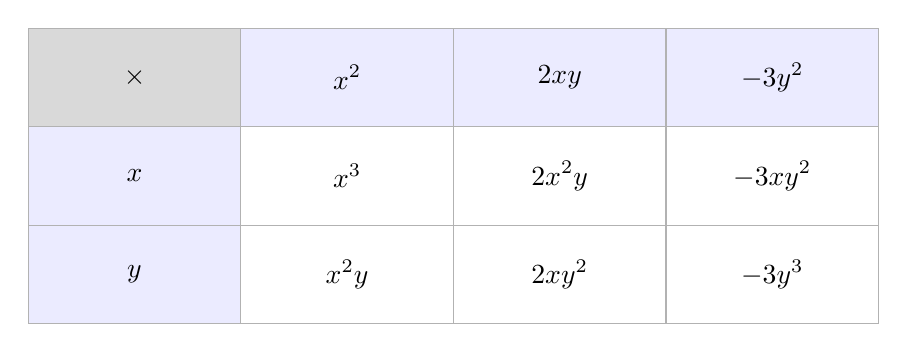
\begin{tikzpicture}[x=1cm,y=1cm]
\fill[gray!30] (0,0) rectangle (2.7,-1.25);
\draw[gray!60] (0,0) rectangle (2.7,-1.25);
\node at (1.35,-0.625) {$\displaystyle \times$};
\fill[blue!8] (2.7,0) rectangle (5.4,-1.25);
\draw[gray!60] (2.7,0) rectangle (5.4,-1.25);
\node at (4.05,-0.625) {$\displaystyle x^2$};
\fill[blue!8] (5.4,0) rectangle (8.1,-1.25);
\draw[gray!60] (5.4,0) rectangle (8.1,-1.25);
\node at (6.75,-0.625) {$\displaystyle 2xy$};
\fill[blue!8] (8.1,0) rectangle (10.8,-1.25);
\draw[gray!60] (8.1,0) rectangle (10.8,-1.25);
\node at (9.45,-0.625) {$\displaystyle -3y^2$};
\fill[blue!8] (0,-1.25) rectangle (2.7,-2.5);
\draw[gray!60] (0,-1.25) rectangle (2.7,-2.5);
\node at (1.35,-1.875) {$\displaystyle x$};
\fill[white] (2.7,-1.25) rectangle (5.4,-2.5);
\draw[gray!60] (2.7,-1.25) rectangle (5.4,-2.5);
\node at (4.05,-1.875) {$\displaystyle x^3$};
\fill[white] (5.4,-1.25) rectangle (8.1,-2.5);
\draw[gray!60] (5.4,-1.25) rectangle (8.1,-2.5);
\node at (6.75,-1.875) {$\displaystyle 2x^2y$};
\fill[white] (8.1,-1.25) rectangle (10.8,-2.5);
\draw[gray!60] (8.1,-1.25) rectangle (10.8,-2.5);
\node at (9.45,-1.875) {$\displaystyle -3xy^2$};
\fill[blue!8] (0,-2.5) rectangle (2.7,-3.75);
\draw[gray!60] (0,-2.5) rectangle (2.7,-3.75);
\node at (1.35,-3.125) {$\displaystyle y$};
\fill[white] (2.7,-2.5) rectangle (5.4,-3.75);
\draw[gray!60] (2.7,-2.5) rectangle (5.4,-3.75);
\node at (4.05,-3.125) {$\displaystyle x^2y$};
\fill[white] (5.4,-2.5) rectangle (8.1,-3.75);
\draw[gray!60] (5.4,-2.5) rectangle (8.1,-3.75);
\node at (6.75,-3.125) {$\displaystyle 2xy^2$};
\fill[white] (8.1,-2.5) rectangle (10.8,-3.75);
\draw[gray!60] (8.1,-2.5) rectangle (10.8,-3.75);
\node at (9.45,-3.125) {$\displaystyle -3y^3$};
\end{tikzpicture}
\end{center}
\small Grid for $(x+y)(x^2+2xy-3y^2)$; every term is then multiplied by the outer factor $xy^3$.\normalsize

\medskip\hrule

\section*{Expanding Brackets 05\quad\small\texttt{(a1-005)}}
\addcontentsline{toc}{section}{Expanding Brackets 05 (a1-005)}
\textit{Difficulty: Foundation \quad\textbar\quad Marks: 4}

\question{Expand \(\Big(x+xy+\frac{x^2}{y}\Big)\Big(x^2-\frac{y}{x^2}+y^2\Big)\).}

\textbf{Worked solution.}

\textit{Expand the brackets}
\[\begin{gathered}
\text{Expand the brackets:} \\[1em] \begin{aligned} &\Big(x+xy+\frac{x^2}{y}\Big)\Big(x^2-\frac{y}{x^2}+y^2\Big) \\ &= x\left(x^2-\frac{y}{x^2}+y^2\right) + xy\left(x^2-\frac{y}{x^2}+y^2\right) + \frac{x^2}{y}\left(x^2-\frac{y}{x^2}+y^2\right) \\ &= x^3-\frac{y}{x}+xy^2 + x^3y-\frac{y^2}{x}+xy^3 + \frac{x^4}{y}-1+x^2y \\ &= x^3 + x^3y + x^2y + xy^2 + xy^3 + \frac{x^4}{y} - \frac{y}{x} - \frac{y^2}{x} - 1 \end{aligned}
\end{gathered}\]
Multiply each term in the first bracket by each term in the second, then collect like terms.

\begin{answerbox}
\textbf{Final answer:}\quad \(\displaystyle x^3 + x^3y + x^2y + xy^2 + xy^3 + \frac{x^4}{y} - \frac{y}{x} - \frac{y^2}{x} - 1\)
\end{answerbox}
\textbf{Area-model diagram.}

\begin{center}
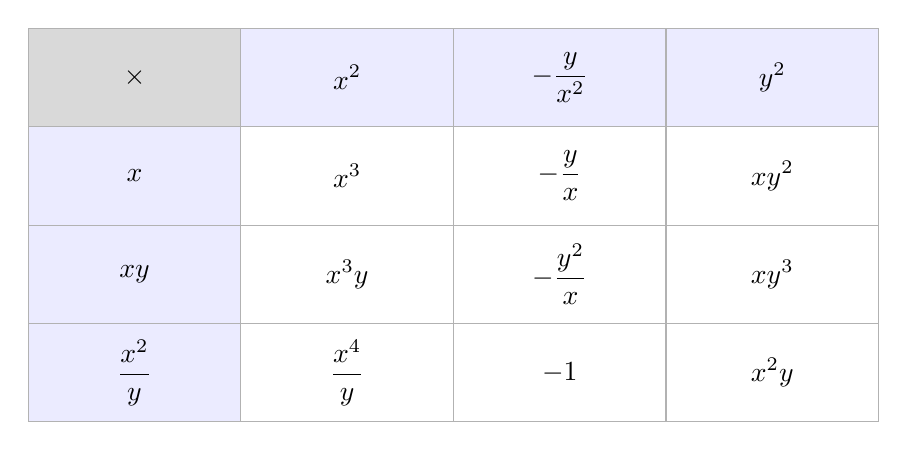
\begin{tikzpicture}[x=1cm,y=1cm]
\fill[gray!30] (0,0) rectangle (2.7,-1.25);
\draw[gray!60] (0,0) rectangle (2.7,-1.25);
\node at (1.35,-0.625) {$\displaystyle \times$};
\fill[blue!8] (2.7,0) rectangle (5.4,-1.25);
\draw[gray!60] (2.7,0) rectangle (5.4,-1.25);
\node at (4.05,-0.625) {$\displaystyle x^2$};
\fill[blue!8] (5.4,0) rectangle (8.1,-1.25);
\draw[gray!60] (5.4,0) rectangle (8.1,-1.25);
\node at (6.75,-0.625) {$\displaystyle -\frac{y}{x^2}$};
\fill[blue!8] (8.1,0) rectangle (10.8,-1.25);
\draw[gray!60] (8.1,0) rectangle (10.8,-1.25);
\node at (9.45,-0.625) {$\displaystyle y^2$};
\fill[blue!8] (0,-1.25) rectangle (2.7,-2.5);
\draw[gray!60] (0,-1.25) rectangle (2.7,-2.5);
\node at (1.35,-1.875) {$\displaystyle x$};
\fill[white] (2.7,-1.25) rectangle (5.4,-2.5);
\draw[gray!60] (2.7,-1.25) rectangle (5.4,-2.5);
\node at (4.05,-1.875) {$\displaystyle x^3$};
\fill[white] (5.4,-1.25) rectangle (8.1,-2.5);
\draw[gray!60] (5.4,-1.25) rectangle (8.1,-2.5);
\node at (6.75,-1.875) {$\displaystyle -\frac{y}{x}$};
\fill[white] (8.1,-1.25) rectangle (10.8,-2.5);
\draw[gray!60] (8.1,-1.25) rectangle (10.8,-2.5);
\node at (9.45,-1.875) {$\displaystyle xy^2$};
\fill[blue!8] (0,-2.5) rectangle (2.7,-3.75);
\draw[gray!60] (0,-2.5) rectangle (2.7,-3.75);
\node at (1.35,-3.125) {$\displaystyle xy$};
\fill[white] (2.7,-2.5) rectangle (5.4,-3.75);
\draw[gray!60] (2.7,-2.5) rectangle (5.4,-3.75);
\node at (4.05,-3.125) {$\displaystyle x^3y$};
\fill[white] (5.4,-2.5) rectangle (8.1,-3.75);
\draw[gray!60] (5.4,-2.5) rectangle (8.1,-3.75);
\node at (6.75,-3.125) {$\displaystyle -\frac{y^2}{x}$};
\fill[white] (8.1,-2.5) rectangle (10.8,-3.75);
\draw[gray!60] (8.1,-2.5) rectangle (10.8,-3.75);
\node at (9.45,-3.125) {$\displaystyle xy^3$};
\fill[blue!8] (0,-3.75) rectangle (2.7,-5);
\draw[gray!60] (0,-3.75) rectangle (2.7,-5);
\node at (1.35,-4.375) {$\displaystyle \frac{x^2}{y}$};
\fill[white] (2.7,-3.75) rectangle (5.4,-5);
\draw[gray!60] (2.7,-3.75) rectangle (5.4,-5);
\node at (4.05,-4.375) {$\displaystyle \frac{x^4}{y}$};
\fill[white] (5.4,-3.75) rectangle (8.1,-5);
\draw[gray!60] (5.4,-3.75) rectangle (8.1,-5);
\node at (6.75,-4.375) {$\displaystyle -1$};
\fill[white] (8.1,-3.75) rectangle (10.8,-5);
\draw[gray!60] (8.1,-3.75) rectangle (10.8,-5);
\node at (9.45,-4.375) {$\displaystyle x^2y$};
\end{tikzpicture}
\end{center}
\medskip\hrule

\section*{Expanding Brackets 06\quad\small\texttt{(a1-006)}}
\addcontentsline{toc}{section}{Expanding Brackets 06 (a1-006)}
\textit{Difficulty: Foundation \quad\textbar\quad Marks: 4}

\question{Expand \(4x - \Big(3(x-2) - 4(2x+3(x-3))\Big)\).}

\textbf{Worked solution.}

\textit{Expand the brackets}
\[\begin{gathered}
\text{Expand the brackets:} \\[1em] \begin{aligned} & 4x - \Big(3(x-2) - 4(2x+3(x-3))\Big) \\ &= 4x - \Big(3x-6 - 4(2x+3x-9)\Big) \\ &= 4x - \Big(3x-6 - 4(5x-9)\Big) \\ &= 4x - \Big(3x-6-20x+36\Big) \\ &= 4x - \Big(-17x+30\Big) \\ &= 4x + 17x - 30 \\ &= 21x - 30 \end{aligned}
\end{gathered}\]
Start by expanding the innermost brackets, then work outwards, simplifying at each step.

\begin{answerbox}
\textbf{Final answer:}\quad \(\displaystyle 21x - 30\)
\end{answerbox}
\textbf{Area-model diagram.}

\begin{center}
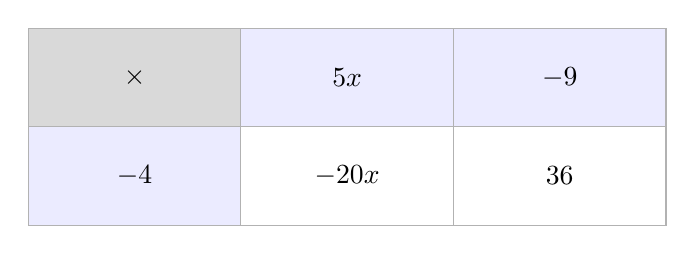
\begin{tikzpicture}[x=1cm,y=1cm]
\fill[gray!30] (0,0) rectangle (2.7,-1.25);
\draw[gray!60] (0,0) rectangle (2.7,-1.25);
\node at (1.35,-0.625) {$\displaystyle \times$};
\fill[blue!8] (2.7,0) rectangle (5.4,-1.25);
\draw[gray!60] (2.7,0) rectangle (5.4,-1.25);
\node at (4.05,-0.625) {$\displaystyle 5x$};
\fill[blue!8] (5.4,0) rectangle (8.1,-1.25);
\draw[gray!60] (5.4,0) rectangle (8.1,-1.25);
\node at (6.75,-0.625) {$\displaystyle -9$};
\fill[blue!8] (0,-1.25) rectangle (2.7,-2.5);
\draw[gray!60] (0,-1.25) rectangle (2.7,-2.5);
\node at (1.35,-1.875) {$\displaystyle -4$};
\fill[white] (2.7,-1.25) rectangle (5.4,-2.5);
\draw[gray!60] (2.7,-1.25) rectangle (5.4,-2.5);
\node at (4.05,-1.875) {$\displaystyle -20x$};
\fill[white] (5.4,-1.25) rectangle (8.1,-2.5);
\draw[gray!60] (5.4,-1.25) rectangle (8.1,-2.5);
\node at (6.75,-1.875) {$\displaystyle 36$};
\end{tikzpicture}
\end{center}
\small Key step: distributing $-4$ over the simplified inner bracket $(5x-9)$.\normalsize

\medskip\hrule

\section*{Expanding Brackets 07\quad\small\texttt{(a1-007)}}
\addcontentsline{toc}{section}{Expanding Brackets 07 (a1-007)}
\textit{Difficulty: Foundation \quad\textbar\quad Marks: 4}

\question{Expand \(  (a+b-c)(a-b+c) + (b+c-a)(b-c+a) \).}

\textbf{Worked solution.}

\textit{Expand the brackets}
\[\begin{gathered}
\begin{aligned} &(a+b-c)(a-b+c)+(b+c-a)(b-c+a) \\ &= (a+(b-c))(a-(b-c))+(b+(c-a))(b-(c-a)) \\ &= a^2-(b-c)^2+b^2-(c-a)^2 \\ &= a^2-(b^2-2bc+c^2)+b^2-(c^2-2ac+a^2) \\ &= a^2-b^2+2bc-c^2+b^2-c^2+2ac-a^2 \\ &= 2bc-2c^2+2ac \\ &= 2c(a+b-c) \end{aligned}
\end{gathered}\]
Recognise that (a+b-c)(a-b+c) = a²-(b-c)² using the difference of two squares. Similarly for the second pair. Then expand and collect like terms.

\begin{answerbox}
\textbf{Final answer:}\quad \(\displaystyle 2c(a+b-c)\)
\end{answerbox}
\textbf{Area-model diagram.}

\begin{center}
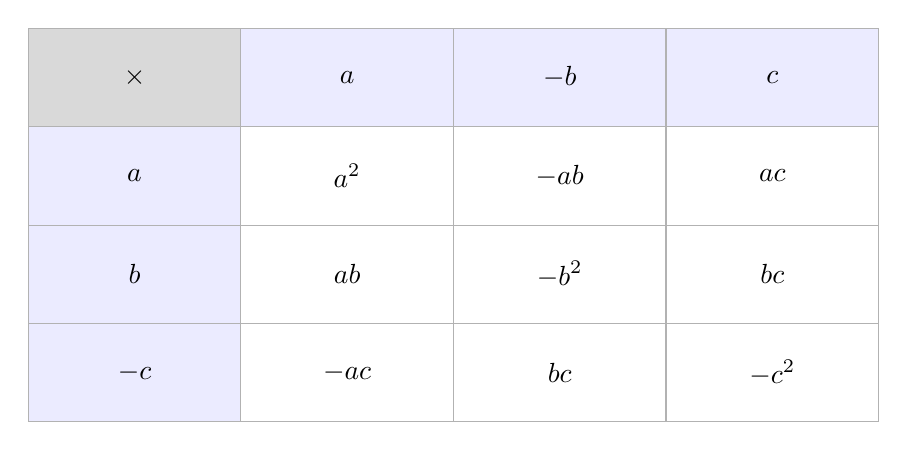
\begin{tikzpicture}[x=1cm,y=1cm]
\fill[gray!30] (0,0) rectangle (2.7,-1.25);
\draw[gray!60] (0,0) rectangle (2.7,-1.25);
\node at (1.35,-0.625) {$\displaystyle \times$};
\fill[blue!8] (2.7,0) rectangle (5.4,-1.25);
\draw[gray!60] (2.7,0) rectangle (5.4,-1.25);
\node at (4.05,-0.625) {$\displaystyle a$};
\fill[blue!8] (5.4,0) rectangle (8.1,-1.25);
\draw[gray!60] (5.4,0) rectangle (8.1,-1.25);
\node at (6.75,-0.625) {$\displaystyle -b$};
\fill[blue!8] (8.1,0) rectangle (10.8,-1.25);
\draw[gray!60] (8.1,0) rectangle (10.8,-1.25);
\node at (9.45,-0.625) {$\displaystyle c$};
\fill[blue!8] (0,-1.25) rectangle (2.7,-2.5);
\draw[gray!60] (0,-1.25) rectangle (2.7,-2.5);
\node at (1.35,-1.875) {$\displaystyle a$};
\fill[white] (2.7,-1.25) rectangle (5.4,-2.5);
\draw[gray!60] (2.7,-1.25) rectangle (5.4,-2.5);
\node at (4.05,-1.875) {$\displaystyle a^2$};
\fill[white] (5.4,-1.25) rectangle (8.1,-2.5);
\draw[gray!60] (5.4,-1.25) rectangle (8.1,-2.5);
\node at (6.75,-1.875) {$\displaystyle -ab$};
\fill[white] (8.1,-1.25) rectangle (10.8,-2.5);
\draw[gray!60] (8.1,-1.25) rectangle (10.8,-2.5);
\node at (9.45,-1.875) {$\displaystyle ac$};
\fill[blue!8] (0,-2.5) rectangle (2.7,-3.75);
\draw[gray!60] (0,-2.5) rectangle (2.7,-3.75);
\node at (1.35,-3.125) {$\displaystyle b$};
\fill[white] (2.7,-2.5) rectangle (5.4,-3.75);
\draw[gray!60] (2.7,-2.5) rectangle (5.4,-3.75);
\node at (4.05,-3.125) {$\displaystyle ab$};
\fill[white] (5.4,-2.5) rectangle (8.1,-3.75);
\draw[gray!60] (5.4,-2.5) rectangle (8.1,-3.75);
\node at (6.75,-3.125) {$\displaystyle -b^2$};
\fill[white] (8.1,-2.5) rectangle (10.8,-3.75);
\draw[gray!60] (8.1,-2.5) rectangle (10.8,-3.75);
\node at (9.45,-3.125) {$\displaystyle bc$};
\fill[blue!8] (0,-3.75) rectangle (2.7,-5);
\draw[gray!60] (0,-3.75) rectangle (2.7,-5);
\node at (1.35,-4.375) {$\displaystyle -c$};
\fill[white] (2.7,-3.75) rectangle (5.4,-5);
\draw[gray!60] (2.7,-3.75) rectangle (5.4,-5);
\node at (4.05,-4.375) {$\displaystyle -ac$};
\fill[white] (5.4,-3.75) rectangle (8.1,-5);
\draw[gray!60] (5.4,-3.75) rectangle (8.1,-5);
\node at (6.75,-4.375) {$\displaystyle bc$};
\fill[white] (8.1,-3.75) rectangle (10.8,-5);
\draw[gray!60] (8.1,-3.75) rectangle (10.8,-5);
\node at (9.45,-4.375) {$\displaystyle -c^2$};
\end{tikzpicture}
\end{center}
\small Grid for the first product $(a+b-c)(a-b+c)$; the second product is handled the same way.\normalsize

\medskip\hrule

\section*{Expanding Brackets 08\quad\small\texttt{(a1-008)}}
\addcontentsline{toc}{section}{Expanding Brackets 08 (a1-008)}
\textit{Difficulty: Foundation \quad\textbar\quad Marks: 4}

\question{Expand \(  (2x-3y^2)^3 \).}

\textbf{Worked solution.}

\textit{Expand step by step, showing each term multiplying out}
\[\begin{gathered}
\begin{aligned} (2x-3y^2)^3 &= (2x-3y^2)\Big[(2x-3y^2)(2x-3y^2)\Big] \\ &= (2x-3y^2)\Big[2x(2x-3y^2)-3y^2(2x-3y^2)\Big] \\ &= (2x-3y^2)\Big[4x^2-6xy^2-6xy^2+9y^4\Big] \\ &= (2x-3y^2)(4x^2-12xy^2+9y^4) \\ &= 2x(4x^2-12xy^2+9y^4)-3y^2(4x^2-12xy^2+9y^4) \\ &= 8x^3-24x^2y^2+18xy^4-12x^2y^2+36xy^4-27y^6 \\ &= 8x^3-36x^2y^2+54xy^4-27y^6 \end{aligned}
\end{gathered}\]
First expand the inner two brackets showing a(c+d)+b(c+d), collect like terms, then multiply the result by the remaining bracket using the same method.

\begin{answerbox}
\textbf{Final answer:}\quad \(\displaystyle 8x^3-36x^2y^2+54xy^4-27y^6\)
\end{answerbox}
\textbf{Area-model diagram.}

\begin{center}
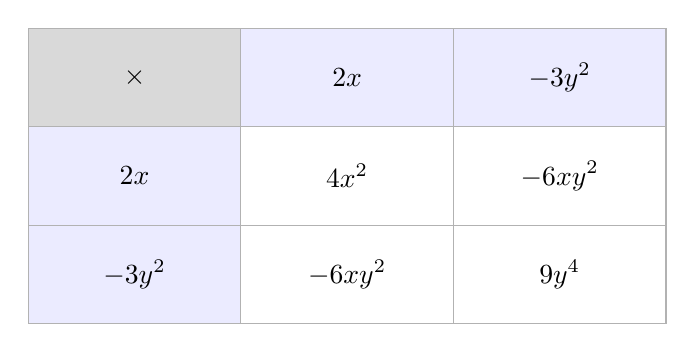
\begin{tikzpicture}[x=1cm,y=1cm]
\fill[gray!30] (0,0) rectangle (2.7,-1.25);
\draw[gray!60] (0,0) rectangle (2.7,-1.25);
\node at (1.35,-0.625) {$\displaystyle \times$};
\fill[blue!8] (2.7,0) rectangle (5.4,-1.25);
\draw[gray!60] (2.7,0) rectangle (5.4,-1.25);
\node at (4.05,-0.625) {$\displaystyle 2x$};
\fill[blue!8] (5.4,0) rectangle (8.1,-1.25);
\draw[gray!60] (5.4,0) rectangle (8.1,-1.25);
\node at (6.75,-0.625) {$\displaystyle -3y^2$};
\fill[blue!8] (0,-1.25) rectangle (2.7,-2.5);
\draw[gray!60] (0,-1.25) rectangle (2.7,-2.5);
\node at (1.35,-1.875) {$\displaystyle 2x$};
\fill[white] (2.7,-1.25) rectangle (5.4,-2.5);
\draw[gray!60] (2.7,-1.25) rectangle (5.4,-2.5);
\node at (4.05,-1.875) {$\displaystyle 4x^2$};
\fill[white] (5.4,-1.25) rectangle (8.1,-2.5);
\draw[gray!60] (5.4,-1.25) rectangle (8.1,-2.5);
\node at (6.75,-1.875) {$\displaystyle -6xy^2$};
\fill[blue!8] (0,-2.5) rectangle (2.7,-3.75);
\draw[gray!60] (0,-2.5) rectangle (2.7,-3.75);
\node at (1.35,-3.125) {$\displaystyle -3y^2$};
\fill[white] (2.7,-2.5) rectangle (5.4,-3.75);
\draw[gray!60] (2.7,-2.5) rectangle (5.4,-3.75);
\node at (4.05,-3.125) {$\displaystyle -6xy^2$};
\fill[white] (5.4,-2.5) rectangle (8.1,-3.75);
\draw[gray!60] (5.4,-2.5) rectangle (8.1,-3.75);
\node at (6.75,-3.125) {$\displaystyle 9y^4$};
\end{tikzpicture}
\end{center}
\small Grid for $(2x-3y^2)^2$; the result $(4x^2-12xy^2+9y^4)$ is then multiplied by $(2x-3y^2)$ again.\normalsize

\medskip\hrule

\section*{Expanding Brackets 09\quad\small\texttt{(a1-009)}}
\addcontentsline{toc}{section}{Expanding Brackets 09 (a1-009)}
\textit{Difficulty: Foundation \quad\textbar\quad Marks: 4}

\question{Expand \(  (m+n)(m^3-mn^2+n^3) \).}

\textbf{Worked solution.}

\textit{Expand the brackets}
\[\begin{gathered}
\text{Expand the brackets:} \\[1em] \begin{aligned} (m+n)(m^3-mn^2+n^3) & = m(m^3-mn^2+n^3)+n(m^3-mn^2+n^3) \\ &= m^4-m^2n^2+mn^3+m^3n-mn^3+n^4 \\ &= m^4+m^3n-m^2n^2+n^4 \end{aligned}
\end{gathered}\]
Expand the first term in the first bracket with the last bracket, and then the second term in the first bracket with the last bracket.

\begin{answerbox}
\textbf{Final answer:}\quad \(\displaystyle m^4+m^3n-m^2n^2+n^4\)
\end{answerbox}
\textbf{Area-model diagram.}

\begin{center}
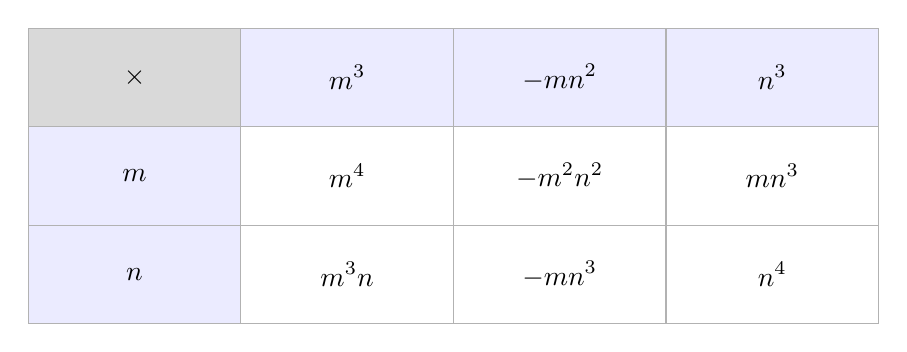
\begin{tikzpicture}[x=1cm,y=1cm]
\fill[gray!30] (0,0) rectangle (2.7,-1.25);
\draw[gray!60] (0,0) rectangle (2.7,-1.25);
\node at (1.35,-0.625) {$\displaystyle \times$};
\fill[blue!8] (2.7,0) rectangle (5.4,-1.25);
\draw[gray!60] (2.7,0) rectangle (5.4,-1.25);
\node at (4.05,-0.625) {$\displaystyle m^3$};
\fill[blue!8] (5.4,0) rectangle (8.1,-1.25);
\draw[gray!60] (5.4,0) rectangle (8.1,-1.25);
\node at (6.75,-0.625) {$\displaystyle -mn^2$};
\fill[blue!8] (8.1,0) rectangle (10.8,-1.25);
\draw[gray!60] (8.1,0) rectangle (10.8,-1.25);
\node at (9.45,-0.625) {$\displaystyle n^3$};
\fill[blue!8] (0,-1.25) rectangle (2.7,-2.5);
\draw[gray!60] (0,-1.25) rectangle (2.7,-2.5);
\node at (1.35,-1.875) {$\displaystyle m$};
\fill[white] (2.7,-1.25) rectangle (5.4,-2.5);
\draw[gray!60] (2.7,-1.25) rectangle (5.4,-2.5);
\node at (4.05,-1.875) {$\displaystyle m^4$};
\fill[white] (5.4,-1.25) rectangle (8.1,-2.5);
\draw[gray!60] (5.4,-1.25) rectangle (8.1,-2.5);
\node at (6.75,-1.875) {$\displaystyle -m^2n^2$};
\fill[white] (8.1,-1.25) rectangle (10.8,-2.5);
\draw[gray!60] (8.1,-1.25) rectangle (10.8,-2.5);
\node at (9.45,-1.875) {$\displaystyle mn^3$};
\fill[blue!8] (0,-2.5) rectangle (2.7,-3.75);
\draw[gray!60] (0,-2.5) rectangle (2.7,-3.75);
\node at (1.35,-3.125) {$\displaystyle n$};
\fill[white] (2.7,-2.5) rectangle (5.4,-3.75);
\draw[gray!60] (2.7,-2.5) rectangle (5.4,-3.75);
\node at (4.05,-3.125) {$\displaystyle m^3n$};
\fill[white] (5.4,-2.5) rectangle (8.1,-3.75);
\draw[gray!60] (5.4,-2.5) rectangle (8.1,-3.75);
\node at (6.75,-3.125) {$\displaystyle -mn^3$};
\fill[white] (8.1,-2.5) rectangle (10.8,-3.75);
\draw[gray!60] (8.1,-2.5) rectangle (10.8,-3.75);
\node at (9.45,-3.125) {$\displaystyle n^4$};
\end{tikzpicture}
\end{center}
\medskip\hrule

\section*{Expanding Brackets 10\quad\small\texttt{(a1-010)}}
\addcontentsline{toc}{section}{Expanding Brackets 10 (a1-010)}
\textit{Difficulty: Foundation \quad\textbar\quad Marks: 4}

\question{Expand \(  pq(q^2-2p+3q)+rs(r^2-2s+3r) \).}

\textbf{Worked solution.}

\textit{Expand the brackets}
\[\begin{gathered}
\text{Expand the brackets:} \\[1em] \begin{aligned} pq(q^2-2p+3q)+rs(r^2-2s+3r) & = pq^3-2p^2q+3pq^2+r^3s-2rs^2+3r^2s \end{aligned}
\end{gathered}\]
Expand each bracket separately, then collect like terms.

\begin{answerbox}
\textbf{Final answer:}\quad \(\displaystyle pq^3-2p^2q+3pq^2+r^3s-2rs^2+3r^2s\)
\end{answerbox}
\textbf{Area-model diagram.}

\begin{center}
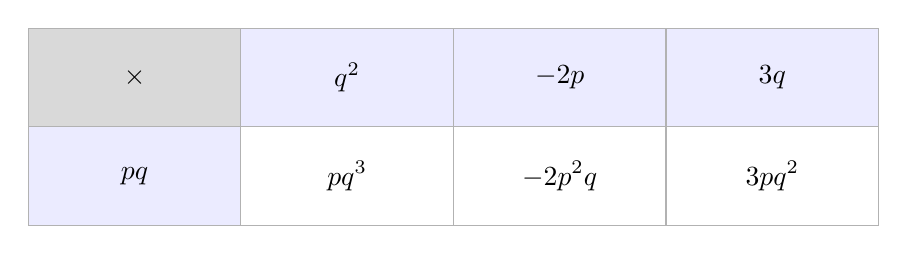
\begin{tikzpicture}[x=1cm,y=1cm]
\fill[gray!30] (0,0) rectangle (2.7,-1.25);
\draw[gray!60] (0,0) rectangle (2.7,-1.25);
\node at (1.35,-0.625) {$\displaystyle \times$};
\fill[blue!8] (2.7,0) rectangle (5.4,-1.25);
\draw[gray!60] (2.7,0) rectangle (5.4,-1.25);
\node at (4.05,-0.625) {$\displaystyle q^2$};
\fill[blue!8] (5.4,0) rectangle (8.1,-1.25);
\draw[gray!60] (5.4,0) rectangle (8.1,-1.25);
\node at (6.75,-0.625) {$\displaystyle -2p$};
\fill[blue!8] (8.1,0) rectangle (10.8,-1.25);
\draw[gray!60] (8.1,0) rectangle (10.8,-1.25);
\node at (9.45,-0.625) {$\displaystyle 3q$};
\fill[blue!8] (0,-1.25) rectangle (2.7,-2.5);
\draw[gray!60] (0,-1.25) rectangle (2.7,-2.5);
\node at (1.35,-1.875) {$\displaystyle pq$};
\fill[white] (2.7,-1.25) rectangle (5.4,-2.5);
\draw[gray!60] (2.7,-1.25) rectangle (5.4,-2.5);
\node at (4.05,-1.875) {$\displaystyle pq^3$};
\fill[white] (5.4,-1.25) rectangle (8.1,-2.5);
\draw[gray!60] (5.4,-1.25) rectangle (8.1,-2.5);
\node at (6.75,-1.875) {$\displaystyle -2p^2q$};
\fill[white] (8.1,-1.25) rectangle (10.8,-2.5);
\draw[gray!60] (8.1,-1.25) rectangle (10.8,-2.5);
\node at (9.45,-1.875) {$\displaystyle 3pq^2$};
\end{tikzpicture}
\end{center}
\small Grid for $pq(q^2-2p+3q)$; the term $rs(r^2-2s+3r)$ expands identically.\normalsize

\medskip\hrule

\section*{Expanding Brackets 11\quad\small\texttt{(a1-011)}}
\addcontentsline{toc}{section}{Expanding Brackets 11 (a1-011)}
\textit{Difficulty: Foundation \quad\textbar\quad Marks: 4}

\question{Expand \(  (x+y+z)(x-y-z) \).}

\textbf{Worked solution.}

\textit{Expand the brackets}
\[\begin{gathered}
\text{Expand the brackets:} \\[1em] \begin{aligned} (x+y+z)(x-y-z) & = x(x-y-z)+y(x-y-z)+z(x-y-z) \\ &= x^2-xy-xz+xy-y^2-yz+xz-yz-z^2 \\ &= x^2-y^2-z^2-2yz \end{aligned}
\end{gathered}\]
Expand each bracket separately, then collect like terms.

\begin{answerbox}
\textbf{Final answer:}\quad \(\displaystyle x^2-y^2-z^2-2yz\)
\end{answerbox}
\textbf{Area-model diagram.}

\begin{center}
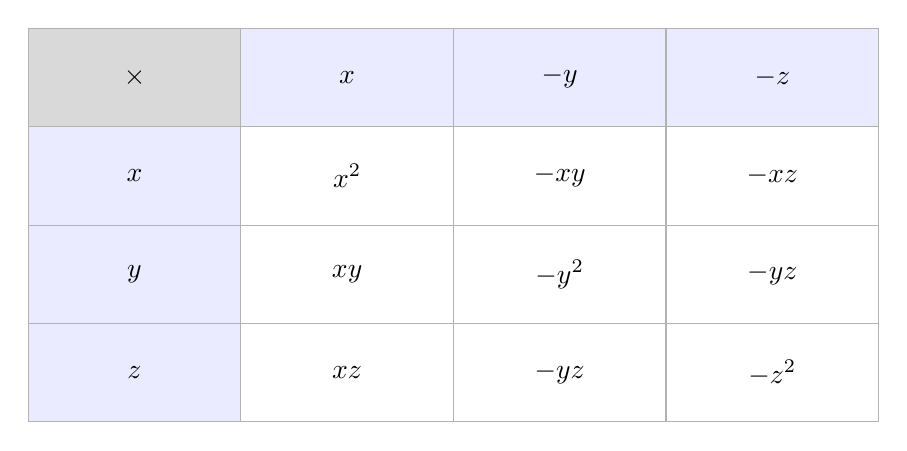
\begin{tikzpicture}[x=1cm,y=1cm]
\fill[gray!30] (0,0) rectangle (2.7,-1.25);
\draw[gray!60] (0,0) rectangle (2.7,-1.25);
\node at (1.35,-0.625) {$\displaystyle \times$};
\fill[blue!8] (2.7,0) rectangle (5.4,-1.25);
\draw[gray!60] (2.7,0) rectangle (5.4,-1.25);
\node at (4.05,-0.625) {$\displaystyle x$};
\fill[blue!8] (5.4,0) rectangle (8.1,-1.25);
\draw[gray!60] (5.4,0) rectangle (8.1,-1.25);
\node at (6.75,-0.625) {$\displaystyle -y$};
\fill[blue!8] (8.1,0) rectangle (10.8,-1.25);
\draw[gray!60] (8.1,0) rectangle (10.8,-1.25);
\node at (9.45,-0.625) {$\displaystyle -z$};
\fill[blue!8] (0,-1.25) rectangle (2.7,-2.5);
\draw[gray!60] (0,-1.25) rectangle (2.7,-2.5);
\node at (1.35,-1.875) {$\displaystyle x$};
\fill[white] (2.7,-1.25) rectangle (5.4,-2.5);
\draw[gray!60] (2.7,-1.25) rectangle (5.4,-2.5);
\node at (4.05,-1.875) {$\displaystyle x^2$};
\fill[white] (5.4,-1.25) rectangle (8.1,-2.5);
\draw[gray!60] (5.4,-1.25) rectangle (8.1,-2.5);
\node at (6.75,-1.875) {$\displaystyle -xy$};
\fill[white] (8.1,-1.25) rectangle (10.8,-2.5);
\draw[gray!60] (8.1,-1.25) rectangle (10.8,-2.5);
\node at (9.45,-1.875) {$\displaystyle -xz$};
\fill[blue!8] (0,-2.5) rectangle (2.7,-3.75);
\draw[gray!60] (0,-2.5) rectangle (2.7,-3.75);
\node at (1.35,-3.125) {$\displaystyle y$};
\fill[white] (2.7,-2.5) rectangle (5.4,-3.75);
\draw[gray!60] (2.7,-2.5) rectangle (5.4,-3.75);
\node at (4.05,-3.125) {$\displaystyle xy$};
\fill[white] (5.4,-2.5) rectangle (8.1,-3.75);
\draw[gray!60] (5.4,-2.5) rectangle (8.1,-3.75);
\node at (6.75,-3.125) {$\displaystyle -y^2$};
\fill[white] (8.1,-2.5) rectangle (10.8,-3.75);
\draw[gray!60] (8.1,-2.5) rectangle (10.8,-3.75);
\node at (9.45,-3.125) {$\displaystyle -yz$};
\fill[blue!8] (0,-3.75) rectangle (2.7,-5);
\draw[gray!60] (0,-3.75) rectangle (2.7,-5);
\node at (1.35,-4.375) {$\displaystyle z$};
\fill[white] (2.7,-3.75) rectangle (5.4,-5);
\draw[gray!60] (2.7,-3.75) rectangle (5.4,-5);
\node at (4.05,-4.375) {$\displaystyle xz$};
\fill[white] (5.4,-3.75) rectangle (8.1,-5);
\draw[gray!60] (5.4,-3.75) rectangle (8.1,-5);
\node at (6.75,-4.375) {$\displaystyle -yz$};
\fill[white] (8.1,-3.75) rectangle (10.8,-5);
\draw[gray!60] (8.1,-3.75) rectangle (10.8,-5);
\node at (9.45,-4.375) {$\displaystyle -z^2$};
\end{tikzpicture}
\end{center}
\medskip\hrule

\section*{Expanding Brackets 12\quad\small\texttt{(a1-012)}}
\addcontentsline{toc}{section}{Expanding Brackets 12 (a1-012)}
\textit{Difficulty: Foundation \quad\textbar\quad Marks: 4}

\question{Expand \(  (x+1)(2x-1)^2 + (x-1)(3x-2)^2 \).}

\textbf{Worked solution.}

\textit{Expand the brackets}
\[\begin{gathered}
\begin{aligned} &(x+1)(2x-1)^2 + (x-1)(3x-2)^2 \\ &= (x+1)\Big(2x(2x-1)-1(2x-1)\Big) + (x-1)\Big(3x(3x-2)-2(3x-2)\Big) \\ &= (x+1)(4x^2-4x+1)+(x-1)(9x^2-12x+4) \\ &= x(4x^2-4x+1)+1(4x^2-4x+1)+x(9x^2-12x+4)-1(9x^2-12x+4) \\ &= (4x^3-4x^2+x+4x^2-4x+1)+(9x^3-12x^2+4x-9x^2+12x-4) \\ &= (4x^3-3x+1)+(9x^3-21x^2+16x-4) \\ &= 13x^3-21x^2+13x-3 \end{aligned}
\end{gathered}\]
Expand each squared bracket using a(c+d)+b(c+d), then multiply out and collect like terms.

\begin{answerbox}
\textbf{Final answer:}\quad \(\displaystyle 13x^3-21x^2+13x-3\)
\end{answerbox}
\textbf{Area-model diagram.}

\begin{center}
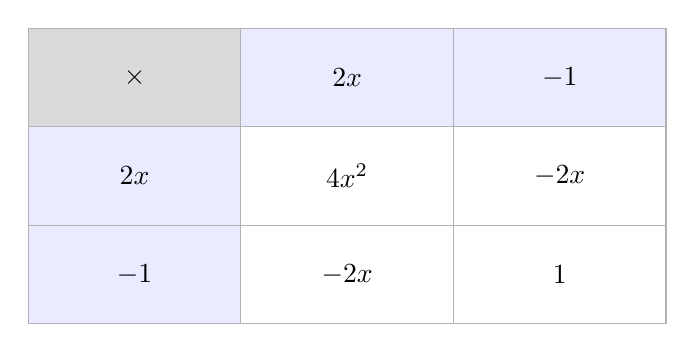
\begin{tikzpicture}[x=1cm,y=1cm]
\fill[gray!30] (0,0) rectangle (2.7,-1.25);
\draw[gray!60] (0,0) rectangle (2.7,-1.25);
\node at (1.35,-0.625) {$\displaystyle \times$};
\fill[blue!8] (2.7,0) rectangle (5.4,-1.25);
\draw[gray!60] (2.7,0) rectangle (5.4,-1.25);
\node at (4.05,-0.625) {$\displaystyle 2x$};
\fill[blue!8] (5.4,0) rectangle (8.1,-1.25);
\draw[gray!60] (5.4,0) rectangle (8.1,-1.25);
\node at (6.75,-0.625) {$\displaystyle -1$};
\fill[blue!8] (0,-1.25) rectangle (2.7,-2.5);
\draw[gray!60] (0,-1.25) rectangle (2.7,-2.5);
\node at (1.35,-1.875) {$\displaystyle 2x$};
\fill[white] (2.7,-1.25) rectangle (5.4,-2.5);
\draw[gray!60] (2.7,-1.25) rectangle (5.4,-2.5);
\node at (4.05,-1.875) {$\displaystyle 4x^2$};
\fill[white] (5.4,-1.25) rectangle (8.1,-2.5);
\draw[gray!60] (5.4,-1.25) rectangle (8.1,-2.5);
\node at (6.75,-1.875) {$\displaystyle -2x$};
\fill[blue!8] (0,-2.5) rectangle (2.7,-3.75);
\draw[gray!60] (0,-2.5) rectangle (2.7,-3.75);
\node at (1.35,-3.125) {$\displaystyle -1$};
\fill[white] (2.7,-2.5) rectangle (5.4,-3.75);
\draw[gray!60] (2.7,-2.5) rectangle (5.4,-3.75);
\node at (4.05,-3.125) {$\displaystyle -2x$};
\fill[white] (5.4,-2.5) rectangle (8.1,-3.75);
\draw[gray!60] (5.4,-2.5) rectangle (8.1,-3.75);
\node at (6.75,-3.125) {$\displaystyle 1$};
\end{tikzpicture}
\end{center}
\small Grid for $(2x-1)^2$; expand $(3x-2)^2$ the same way, then multiply each by its linear factor.\normalsize

\medskip\hrule

\section*{Expanding Brackets 13\quad\small\texttt{(a1-013)}}
\addcontentsline{toc}{section}{Expanding Brackets 13 (a1-013)}
\textit{Difficulty: Foundation \quad\textbar\quad Marks: 4}

\question{Expand \(  (x+2)(3x+1)^2 - (x-1)(2x+3)^2 \).}

\textbf{Worked solution.}

\textit{Expand each squared bracket, then multiply out}
\[\begin{gathered}
\begin{aligned} &(x+2)(3x+1)^2 - (x-1)(2x+3)^2 \\ &= (x+2)\Big(3x(3x+1)+1(3x+1)\Big) - (x-1)\Big(2x(2x+3)+3(2x+3)\Big) \\ &= (x+2)(9x^2+6x+1) - (x-1)(4x^2+12x+9) \\ &= x(9x^2+6x+1)+2(9x^2+6x+1) - \Big[x(4x^2+12x+9)-1(4x^2+12x+9)\Big] \\ &= (9x^3+6x^2+x+18x^2+12x+2) - (4x^3+12x^2+9x-4x^2-12x-9) \\ &= (9x^3+24x^2+13x+2) - (4x^3+8x^2-3x-9) \\ &= 9x^3+24x^2+13x+2-4x^3-8x^2+3x+9 \\ &= 5x^3+16x^2+16x+11 \end{aligned}
\end{gathered}\]
Expand each squared bracket using a(c+d)+b(c+d), multiply out both products, then subtract and collect like terms.

\begin{answerbox}
\textbf{Final answer:}\quad \(\displaystyle 5x^3+16x^2+16x+11\)
\end{answerbox}
\textbf{Area-model diagram.}

\begin{center}
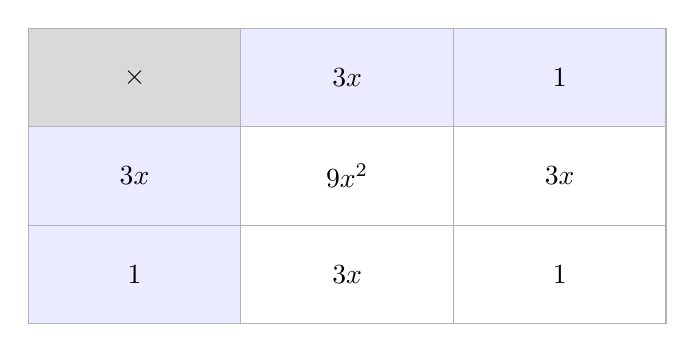
\begin{tikzpicture}[x=1cm,y=1cm]
\fill[gray!30] (0,0) rectangle (2.7,-1.25);
\draw[gray!60] (0,0) rectangle (2.7,-1.25);
\node at (1.35,-0.625) {$\displaystyle \times$};
\fill[blue!8] (2.7,0) rectangle (5.4,-1.25);
\draw[gray!60] (2.7,0) rectangle (5.4,-1.25);
\node at (4.05,-0.625) {$\displaystyle 3x$};
\fill[blue!8] (5.4,0) rectangle (8.1,-1.25);
\draw[gray!60] (5.4,0) rectangle (8.1,-1.25);
\node at (6.75,-0.625) {$\displaystyle 1$};
\fill[blue!8] (0,-1.25) rectangle (2.7,-2.5);
\draw[gray!60] (0,-1.25) rectangle (2.7,-2.5);
\node at (1.35,-1.875) {$\displaystyle 3x$};
\fill[white] (2.7,-1.25) rectangle (5.4,-2.5);
\draw[gray!60] (2.7,-1.25) rectangle (5.4,-2.5);
\node at (4.05,-1.875) {$\displaystyle 9x^2$};
\fill[white] (5.4,-1.25) rectangle (8.1,-2.5);
\draw[gray!60] (5.4,-1.25) rectangle (8.1,-2.5);
\node at (6.75,-1.875) {$\displaystyle 3x$};
\fill[blue!8] (0,-2.5) rectangle (2.7,-3.75);
\draw[gray!60] (0,-2.5) rectangle (2.7,-3.75);
\node at (1.35,-3.125) {$\displaystyle 1$};
\fill[white] (2.7,-2.5) rectangle (5.4,-3.75);
\draw[gray!60] (2.7,-2.5) rectangle (5.4,-3.75);
\node at (4.05,-3.125) {$\displaystyle 3x$};
\fill[white] (5.4,-2.5) rectangle (8.1,-3.75);
\draw[gray!60] (5.4,-2.5) rectangle (8.1,-3.75);
\node at (6.75,-3.125) {$\displaystyle 1$};
\end{tikzpicture}
\end{center}
\small Grid for $(3x+1)^2$; treat $(2x+3)^2$ the same way.\normalsize

\medskip\hrule

\section*{Expanding Brackets 14\quad\small\texttt{(a1-014)}}
\addcontentsline{toc}{section}{Expanding Brackets 14 (a1-014)}
\textit{Difficulty: Foundation \quad\textbar\quad Marks: 4}

\question{Expand \( (3a+2b)^2 - (3a-2b)^2 \).}

\textbf{Worked solution.}

\textit{Expand the squares and simplify}
\[\begin{gathered}
\text{Expand the brackets:} \\[1em] \begin{aligned} (3a+2b)^2 - (3a-2b)^2 & = (3a+2b)(3a+2b) - (3a-2b)(3a-2b) \\ &= 3a(3a+2b)+2b(3a+2b) - 3a(3a-2b)-2b(3a-2b) \\ &= 9a^2 + 6ab + 6ab + 4b^2 - (9a^2 - 6ab - 6ab + 4b^2) \\ &= 9a^2 + 12ab + 4b^2 - (9a^2 - 12ab + 4b^2) \\ &= 9a^2 + 12ab + 4b^2 - 9a^2 + 12ab - 4b^2 \\ &= 24ab \end{aligned}
\end{gathered}\]
Expand both squared binomials separately, then subtract the second expansion from the first, taking care with the signs.

\begin{answerbox}
\textbf{Final answer:}\quad \(\displaystyle 24ab\)
\end{answerbox}
\textbf{Area-model diagram.}

\begin{center}
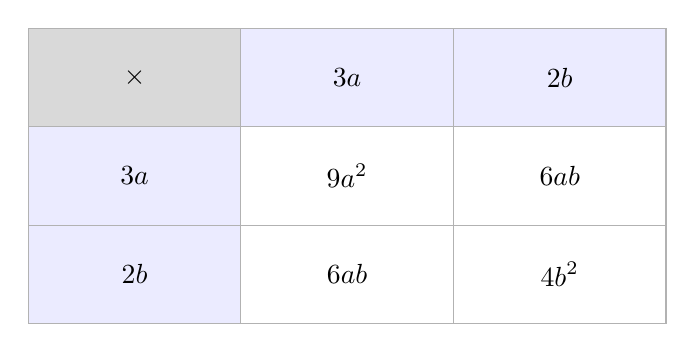
\begin{tikzpicture}[x=1cm,y=1cm]
\fill[gray!30] (0,0) rectangle (2.7,-1.25);
\draw[gray!60] (0,0) rectangle (2.7,-1.25);
\node at (1.35,-0.625) {$\displaystyle \times$};
\fill[blue!8] (2.7,0) rectangle (5.4,-1.25);
\draw[gray!60] (2.7,0) rectangle (5.4,-1.25);
\node at (4.05,-0.625) {$\displaystyle 3a$};
\fill[blue!8] (5.4,0) rectangle (8.1,-1.25);
\draw[gray!60] (5.4,0) rectangle (8.1,-1.25);
\node at (6.75,-0.625) {$\displaystyle 2b$};
\fill[blue!8] (0,-1.25) rectangle (2.7,-2.5);
\draw[gray!60] (0,-1.25) rectangle (2.7,-2.5);
\node at (1.35,-1.875) {$\displaystyle 3a$};
\fill[white] (2.7,-1.25) rectangle (5.4,-2.5);
\draw[gray!60] (2.7,-1.25) rectangle (5.4,-2.5);
\node at (4.05,-1.875) {$\displaystyle 9a^2$};
\fill[white] (5.4,-1.25) rectangle (8.1,-2.5);
\draw[gray!60] (5.4,-1.25) rectangle (8.1,-2.5);
\node at (6.75,-1.875) {$\displaystyle 6ab$};
\fill[blue!8] (0,-2.5) rectangle (2.7,-3.75);
\draw[gray!60] (0,-2.5) rectangle (2.7,-3.75);
\node at (1.35,-3.125) {$\displaystyle 2b$};
\fill[white] (2.7,-2.5) rectangle (5.4,-3.75);
\draw[gray!60] (2.7,-2.5) rectangle (5.4,-3.75);
\node at (4.05,-3.125) {$\displaystyle 6ab$};
\fill[white] (5.4,-2.5) rectangle (8.1,-3.75);
\draw[gray!60] (5.4,-2.5) rectangle (8.1,-3.75);
\node at (6.75,-3.125) {$\displaystyle 4b^2$};
\end{tikzpicture}
\end{center}
\small Grid for $(3a+2b)^2$; subtract the analogous grid for $(3a-2b)^2$.\normalsize

\medskip\hrule

\section*{Expanding Brackets 15\quad\small\texttt{(a1-015)}}
\addcontentsline{toc}{section}{Expanding Brackets 15 (a1-015)}
\textit{Difficulty: Foundation \quad\textbar\quad Marks: 4}

\question{Expand \( (x^2+2)(x^2-5x+3) \).}

\textbf{Worked solution.}

\textit{Expand the brackets}
\[\begin{gathered}
\text{Expand the brackets:} \\[1em] \begin{aligned} (x^2+2)(x^2-5x+3) & = x^2(x^2-5x+3) + 2(x^2-5x+3) \\ &= x^2(x^2) +x^2(-5x)+x^2(3) + 2(x^2) + 2(-5x) + 2(3) \\ &= x^4 - 5x^3 + 3x^2 + 2x^2 - 10x + 6 \\ &= x^4 - 5x^3 + 5x^2 - 10x + 6 \end{aligned}
\end{gathered}\]
Distribute each term in the first bracket across the second bracket, then combine the like terms.

\begin{answerbox}
\textbf{Final answer:}\quad \(\displaystyle x^4 - 5x^3 + 5x^2 - 10x + 6\)
\end{answerbox}
\textbf{Area-model diagram.}

\begin{center}
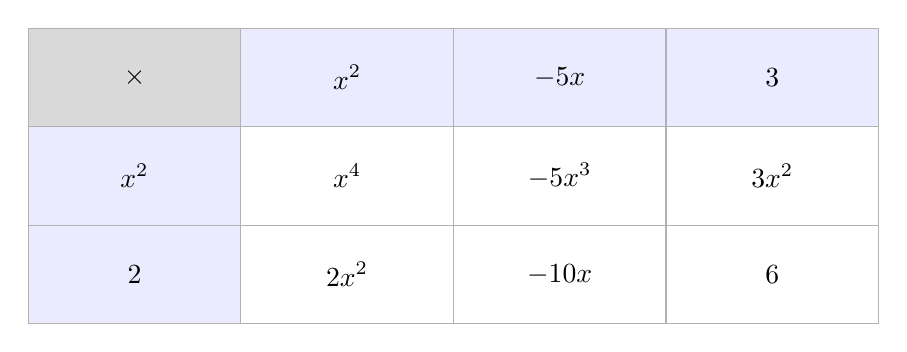
\begin{tikzpicture}[x=1cm,y=1cm]
\fill[gray!30] (0,0) rectangle (2.7,-1.25);
\draw[gray!60] (0,0) rectangle (2.7,-1.25);
\node at (1.35,-0.625) {$\displaystyle \times$};
\fill[blue!8] (2.7,0) rectangle (5.4,-1.25);
\draw[gray!60] (2.7,0) rectangle (5.4,-1.25);
\node at (4.05,-0.625) {$\displaystyle x^2$};
\fill[blue!8] (5.4,0) rectangle (8.1,-1.25);
\draw[gray!60] (5.4,0) rectangle (8.1,-1.25);
\node at (6.75,-0.625) {$\displaystyle -5x$};
\fill[blue!8] (8.1,0) rectangle (10.8,-1.25);
\draw[gray!60] (8.1,0) rectangle (10.8,-1.25);
\node at (9.45,-0.625) {$\displaystyle 3$};
\fill[blue!8] (0,-1.25) rectangle (2.7,-2.5);
\draw[gray!60] (0,-1.25) rectangle (2.7,-2.5);
\node at (1.35,-1.875) {$\displaystyle x^2$};
\fill[white] (2.7,-1.25) rectangle (5.4,-2.5);
\draw[gray!60] (2.7,-1.25) rectangle (5.4,-2.5);
\node at (4.05,-1.875) {$\displaystyle x^4$};
\fill[white] (5.4,-1.25) rectangle (8.1,-2.5);
\draw[gray!60] (5.4,-1.25) rectangle (8.1,-2.5);
\node at (6.75,-1.875) {$\displaystyle -5x^3$};
\fill[white] (8.1,-1.25) rectangle (10.8,-2.5);
\draw[gray!60] (8.1,-1.25) rectangle (10.8,-2.5);
\node at (9.45,-1.875) {$\displaystyle 3x^2$};
\fill[blue!8] (0,-2.5) rectangle (2.7,-3.75);
\draw[gray!60] (0,-2.5) rectangle (2.7,-3.75);
\node at (1.35,-3.125) {$\displaystyle 2$};
\fill[white] (2.7,-2.5) rectangle (5.4,-3.75);
\draw[gray!60] (2.7,-2.5) rectangle (5.4,-3.75);
\node at (4.05,-3.125) {$\displaystyle 2x^2$};
\fill[white] (5.4,-2.5) rectangle (8.1,-3.75);
\draw[gray!60] (5.4,-2.5) rectangle (8.1,-3.75);
\node at (6.75,-3.125) {$\displaystyle -10x$};
\fill[white] (8.1,-2.5) rectangle (10.8,-3.75);
\draw[gray!60] (8.1,-2.5) rectangle (10.8,-3.75);
\node at (9.45,-3.125) {$\displaystyle 6$};
\end{tikzpicture}
\end{center}
\medskip\hrule

\section*{Expanding Brackets 16\quad\small\texttt{(a1-016)}}
\addcontentsline{toc}{section}{Expanding Brackets 16 (a1-016)}
\textit{Difficulty: Foundation \quad\textbar\quad Marks: 4}

\question{Expand \( (a-b)(a+b)(a^2+b^2) \).}

\textbf{Worked solution.}

\textit{Expand the first two brackets}
\[\begin{gathered}
\text{Step 1: Difference of two squares} \\[1em] \begin{aligned} (a-b)(a+b)(a^2+b^2) &= \Big(a(a+b)-b(a+b)\Big)(a^2+b^2) \\ & = \Big( a^2+ab-ba-b^2\Big)(a^2+b^2) \\ & = \Big( a^2-b^2\Big)(a^2+b^2) \\ & = \Big( a^2(a^2+b^2)-b^2(a^2+b^2)\Big) \\ & = a^4+a^2b^2-b^2a^2-b^4 \\ & = a^4-b^4 \end{aligned}
\end{gathered}\]
Recognize that the first two brackets form a difference of two squares.

\begin{answerbox}
\textbf{Final answer:}\quad \(\displaystyle a^4 - b^4\)
\end{answerbox}
\textbf{Area-model diagram.}

\begin{center}
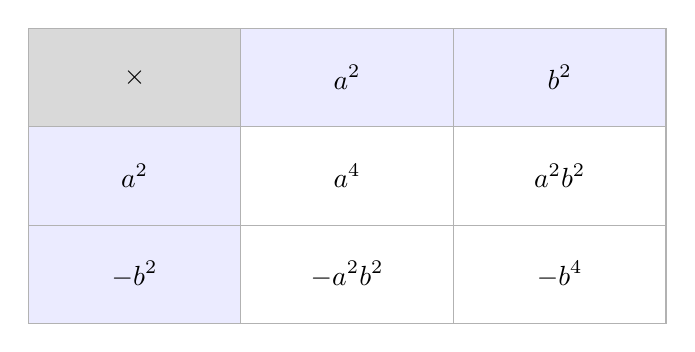
\begin{tikzpicture}[x=1cm,y=1cm]
\fill[gray!30] (0,0) rectangle (2.7,-1.25);
\draw[gray!60] (0,0) rectangle (2.7,-1.25);
\node at (1.35,-0.625) {$\displaystyle \times$};
\fill[blue!8] (2.7,0) rectangle (5.4,-1.25);
\draw[gray!60] (2.7,0) rectangle (5.4,-1.25);
\node at (4.05,-0.625) {$\displaystyle a^2$};
\fill[blue!8] (5.4,0) rectangle (8.1,-1.25);
\draw[gray!60] (5.4,0) rectangle (8.1,-1.25);
\node at (6.75,-0.625) {$\displaystyle b^2$};
\fill[blue!8] (0,-1.25) rectangle (2.7,-2.5);
\draw[gray!60] (0,-1.25) rectangle (2.7,-2.5);
\node at (1.35,-1.875) {$\displaystyle a^2$};
\fill[white] (2.7,-1.25) rectangle (5.4,-2.5);
\draw[gray!60] (2.7,-1.25) rectangle (5.4,-2.5);
\node at (4.05,-1.875) {$\displaystyle a^4$};
\fill[white] (5.4,-1.25) rectangle (8.1,-2.5);
\draw[gray!60] (5.4,-1.25) rectangle (8.1,-2.5);
\node at (6.75,-1.875) {$\displaystyle a^2b^2$};
\fill[blue!8] (0,-2.5) rectangle (2.7,-3.75);
\draw[gray!60] (0,-2.5) rectangle (2.7,-3.75);
\node at (1.35,-3.125) {$\displaystyle -b^2$};
\fill[white] (2.7,-2.5) rectangle (5.4,-3.75);
\draw[gray!60] (2.7,-2.5) rectangle (5.4,-3.75);
\node at (4.05,-3.125) {$\displaystyle -a^2b^2$};
\fill[white] (5.4,-2.5) rectangle (8.1,-3.75);
\draw[gray!60] (5.4,-2.5) rectangle (8.1,-3.75);
\node at (6.75,-3.125) {$\displaystyle -b^4$};
\end{tikzpicture}
\end{center}
\small After $(a-b)(a+b)=a^2-b^2$, this grid multiplies it by $(a^2+b^2)$.\normalsize

\medskip\hrule

\section*{Expanding Brackets 17\quad\small\texttt{(a1-017)}}
\addcontentsline{toc}{section}{Expanding Brackets 17 (a1-017)}
\textit{Difficulty: Foundation \quad\textbar\quad Marks: 4}

\question{Expand \( 2x(x-3)^2 - x^2(2x+1) \).}

\textbf{Worked solution.}

\textit{Expand the squares and distribute}
\[\begin{gathered}
\text{Expand the brackets:} \\[1em] \begin{aligned} 2x(x-3)^2 - x^2(2x+1) & = 2x(x-3)(x-3) - (2x^3+x^2) \\ &= 2x(x(x-3)-3(x-3)) - (2x^3+x^2) \\ &= 2x(x^2-3x-3x+9) - (2x^3+x^2) \\ &= 2x(x^2-6x+9) - (2x^3+x^2) \\ &= 2x^3 - 12x^2 + 18x - 2x^3 - x^2 \\ &= -13x^2 + 18x \end{aligned}
\end{gathered}\]
First square the binomial, then multiply by 2x. Expand the second part and carefully subtract to collect like terms.

\begin{answerbox}
\textbf{Final answer:}\quad \(\displaystyle -13x^2 + 18x\)
\end{answerbox}
\textbf{Area-model diagram.}

\begin{center}
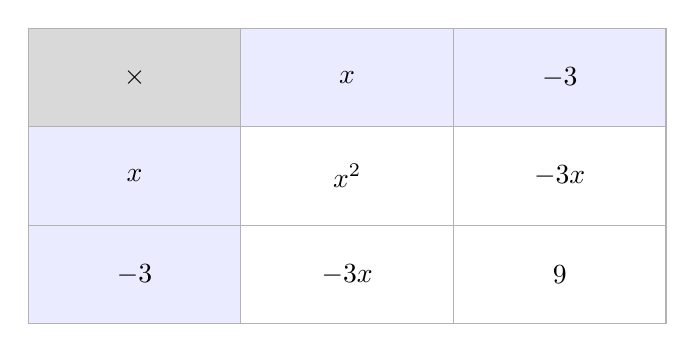
\begin{tikzpicture}[x=1cm,y=1cm]
\fill[gray!30] (0,0) rectangle (2.7,-1.25);
\draw[gray!60] (0,0) rectangle (2.7,-1.25);
\node at (1.35,-0.625) {$\displaystyle \times$};
\fill[blue!8] (2.7,0) rectangle (5.4,-1.25);
\draw[gray!60] (2.7,0) rectangle (5.4,-1.25);
\node at (4.05,-0.625) {$\displaystyle x$};
\fill[blue!8] (5.4,0) rectangle (8.1,-1.25);
\draw[gray!60] (5.4,0) rectangle (8.1,-1.25);
\node at (6.75,-0.625) {$\displaystyle -3$};
\fill[blue!8] (0,-1.25) rectangle (2.7,-2.5);
\draw[gray!60] (0,-1.25) rectangle (2.7,-2.5);
\node at (1.35,-1.875) {$\displaystyle x$};
\fill[white] (2.7,-1.25) rectangle (5.4,-2.5);
\draw[gray!60] (2.7,-1.25) rectangle (5.4,-2.5);
\node at (4.05,-1.875) {$\displaystyle x^2$};
\fill[white] (5.4,-1.25) rectangle (8.1,-2.5);
\draw[gray!60] (5.4,-1.25) rectangle (8.1,-2.5);
\node at (6.75,-1.875) {$\displaystyle -3x$};
\fill[blue!8] (0,-2.5) rectangle (2.7,-3.75);
\draw[gray!60] (0,-2.5) rectangle (2.7,-3.75);
\node at (1.35,-3.125) {$\displaystyle -3$};
\fill[white] (2.7,-2.5) rectangle (5.4,-3.75);
\draw[gray!60] (2.7,-2.5) rectangle (5.4,-3.75);
\node at (4.05,-3.125) {$\displaystyle -3x$};
\fill[white] (5.4,-2.5) rectangle (8.1,-3.75);
\draw[gray!60] (5.4,-2.5) rectangle (8.1,-3.75);
\node at (6.75,-3.125) {$\displaystyle 9$};
\end{tikzpicture}
\end{center}
\small Grid for $(x-3)^2$; the result is then multiplied by $2x$.\normalsize

\medskip\hrule

\section*{Expanding Brackets 18\quad\small\texttt{(a1-018)}}
\addcontentsline{toc}{section}{Expanding Brackets 18 (a1-018)}
\textit{Difficulty: Foundation \quad\textbar\quad Marks: 4}

\question{Expand \( (x+2)(x-3)(x+4) \).}

\textbf{Worked solution.}

\textit{Expand the first two brackets}
\[\begin{gathered}
\text{Expand:} \\[1em] \begin{aligned} (x+2)\Big( (x-3)(x+4)\Big) & = (x+2)\Big(x(x+4)-3(x+4)) \\ &= (x+2)\Big(x^2+4x-3x-12\Big) \\ &= (x+2)\Big(x^2+x-12\Big) \\ &= x(x^2+x-12)+2(x^2+x-12) \\ &= x^3+x^2-12x+2x^2+2x-24 \\ &= x^3+3x^2-10x-24 \end{aligned}
\end{gathered}\]
Multiply the first two terms and simplify.

\begin{answerbox}
\textbf{Final answer:}\quad \(\displaystyle x^3 + 3x^2 - 10x - 24\)
\end{answerbox}
\textbf{Area-model diagram.}

\begin{center}
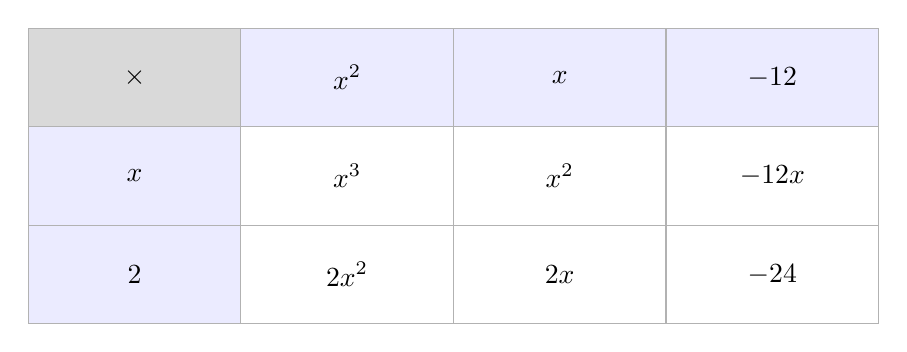
\begin{tikzpicture}[x=1cm,y=1cm]
\fill[gray!30] (0,0) rectangle (2.7,-1.25);
\draw[gray!60] (0,0) rectangle (2.7,-1.25);
\node at (1.35,-0.625) {$\displaystyle \times$};
\fill[blue!8] (2.7,0) rectangle (5.4,-1.25);
\draw[gray!60] (2.7,0) rectangle (5.4,-1.25);
\node at (4.05,-0.625) {$\displaystyle x^2$};
\fill[blue!8] (5.4,0) rectangle (8.1,-1.25);
\draw[gray!60] (5.4,0) rectangle (8.1,-1.25);
\node at (6.75,-0.625) {$\displaystyle x$};
\fill[blue!8] (8.1,0) rectangle (10.8,-1.25);
\draw[gray!60] (8.1,0) rectangle (10.8,-1.25);
\node at (9.45,-0.625) {$\displaystyle -12$};
\fill[blue!8] (0,-1.25) rectangle (2.7,-2.5);
\draw[gray!60] (0,-1.25) rectangle (2.7,-2.5);
\node at (1.35,-1.875) {$\displaystyle x$};
\fill[white] (2.7,-1.25) rectangle (5.4,-2.5);
\draw[gray!60] (2.7,-1.25) rectangle (5.4,-2.5);
\node at (4.05,-1.875) {$\displaystyle x^3$};
\fill[white] (5.4,-1.25) rectangle (8.1,-2.5);
\draw[gray!60] (5.4,-1.25) rectangle (8.1,-2.5);
\node at (6.75,-1.875) {$\displaystyle x^2$};
\fill[white] (8.1,-1.25) rectangle (10.8,-2.5);
\draw[gray!60] (8.1,-1.25) rectangle (10.8,-2.5);
\node at (9.45,-1.875) {$\displaystyle -12x$};
\fill[blue!8] (0,-2.5) rectangle (2.7,-3.75);
\draw[gray!60] (0,-2.5) rectangle (2.7,-3.75);
\node at (1.35,-3.125) {$\displaystyle 2$};
\fill[white] (2.7,-2.5) rectangle (5.4,-3.75);
\draw[gray!60] (2.7,-2.5) rectangle (5.4,-3.75);
\node at (4.05,-3.125) {$\displaystyle 2x^2$};
\fill[white] (5.4,-2.5) rectangle (8.1,-3.75);
\draw[gray!60] (5.4,-2.5) rectangle (8.1,-3.75);
\node at (6.75,-3.125) {$\displaystyle 2x$};
\fill[white] (8.1,-2.5) rectangle (10.8,-3.75);
\draw[gray!60] (8.1,-2.5) rectangle (10.8,-3.75);
\node at (9.45,-3.125) {$\displaystyle -24$};
\end{tikzpicture}
\end{center}
\small After $(x-3)(x+4)=x^2+x-12$, this grid multiplies it by $(x+2)$.\normalsize

\medskip\hrule

\section*{Expanding Brackets 19\quad\small\texttt{(a1-019)}}
\addcontentsline{toc}{section}{Expanding Brackets 19 (a1-019)}
\textit{Difficulty: Foundation \quad\textbar\quad Marks: 3}

\question{A rectangle has a length of \( 2x + 5 \) and a width of \( x - 3 \). Write an expanded expression for the area of the rectangle.}

\textbf{Worked solution.}

\textit{Set up and expand}
\[\begin{gathered}
\begin{aligned} \text{Area} &= (2x + 5)(x - 3) \\ &= 2x(x-3) + 5(x-3) \\ &= 2x^2 - 6x + 5x - 15 \\ &= 2x^2 - x - 15 \end{aligned}
\end{gathered}\]
The area of a rectangle is length times width. Expand the brackets and collect like terms.

\begin{answerbox}
\textbf{Final answer:}\quad \(\displaystyle 2x^2 - x - 15\)
\end{answerbox}
\textbf{Area-model diagram.}

\begin{center}
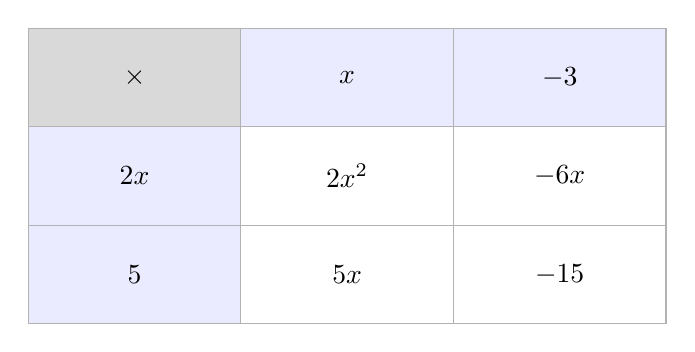
\begin{tikzpicture}[x=1cm,y=1cm]
\fill[gray!30] (0,0) rectangle (2.7,-1.25);
\draw[gray!60] (0,0) rectangle (2.7,-1.25);
\node at (1.35,-0.625) {$\displaystyle \times$};
\fill[blue!8] (2.7,0) rectangle (5.4,-1.25);
\draw[gray!60] (2.7,0) rectangle (5.4,-1.25);
\node at (4.05,-0.625) {$\displaystyle x$};
\fill[blue!8] (5.4,0) rectangle (8.1,-1.25);
\draw[gray!60] (5.4,0) rectangle (8.1,-1.25);
\node at (6.75,-0.625) {$\displaystyle -3$};
\fill[blue!8] (0,-1.25) rectangle (2.7,-2.5);
\draw[gray!60] (0,-1.25) rectangle (2.7,-2.5);
\node at (1.35,-1.875) {$\displaystyle 2x$};
\fill[white] (2.7,-1.25) rectangle (5.4,-2.5);
\draw[gray!60] (2.7,-1.25) rectangle (5.4,-2.5);
\node at (4.05,-1.875) {$\displaystyle 2x^2$};
\fill[white] (5.4,-1.25) rectangle (8.1,-2.5);
\draw[gray!60] (5.4,-1.25) rectangle (8.1,-2.5);
\node at (6.75,-1.875) {$\displaystyle -6x$};
\fill[blue!8] (0,-2.5) rectangle (2.7,-3.75);
\draw[gray!60] (0,-2.5) rectangle (2.7,-3.75);
\node at (1.35,-3.125) {$\displaystyle 5$};
\fill[white] (2.7,-2.5) rectangle (5.4,-3.75);
\draw[gray!60] (2.7,-2.5) rectangle (5.4,-3.75);
\node at (4.05,-3.125) {$\displaystyle 5x$};
\fill[white] (5.4,-2.5) rectangle (8.1,-3.75);
\draw[gray!60] (5.4,-2.5) rectangle (8.1,-3.75);
\node at (6.75,-3.125) {$\displaystyle -15$};
\end{tikzpicture}
\end{center}
\small This is literally the rectangle: length $2x+5$ down the side, width $x-3$ along the top.\normalsize

\medskip\hrule

\section*{Expanding Brackets 20\quad\small\texttt{(a1-020)}}
\addcontentsline{toc}{section}{Expanding Brackets 20 (a1-020)}
\textit{Difficulty: Foundation \quad\textbar\quad Marks: 3}

\question{Expand and simplify \( \frac{1}{4}(12x - 8) - \frac{1}{5}(10x + 5) \).}

\textbf{Worked solution.}

\textit{Expand the brackets using the fractional coefficients}
\[\begin{gathered}
\text{Expand:} \\[1em] \begin{aligned} \frac{1}{4}(12x - 8)-\frac{1}{5}(10x+5) &= 3x-2-2x-1 \\ & = x-3 \end{aligned}
\end{gathered}\]
Divide the first bracket by 4 and the second bracket by 5, being careful to distribute the negative sign.

\begin{answerbox}
\textbf{Final answer:}\quad \(\displaystyle x - 3\)
\end{answerbox}
\textbf{Area-model diagram.}

\begin{center}
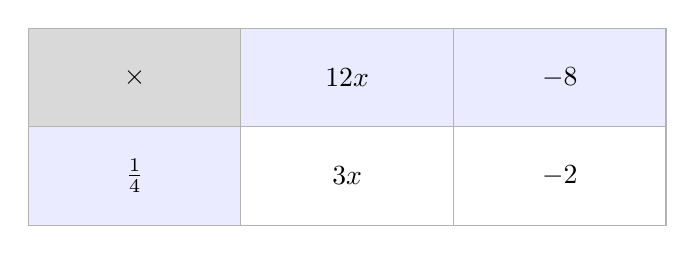
\begin{tikzpicture}[x=1cm,y=1cm]
\fill[gray!30] (0,0) rectangle (2.7,-1.25);
\draw[gray!60] (0,0) rectangle (2.7,-1.25);
\node at (1.35,-0.625) {$\displaystyle \times$};
\fill[blue!8] (2.7,0) rectangle (5.4,-1.25);
\draw[gray!60] (2.7,0) rectangle (5.4,-1.25);
\node at (4.05,-0.625) {$\displaystyle 12x$};
\fill[blue!8] (5.4,0) rectangle (8.1,-1.25);
\draw[gray!60] (5.4,0) rectangle (8.1,-1.25);
\node at (6.75,-0.625) {$\displaystyle -8$};
\fill[blue!8] (0,-1.25) rectangle (2.7,-2.5);
\draw[gray!60] (0,-1.25) rectangle (2.7,-2.5);
\node at (1.35,-1.875) {$\displaystyle \tfrac{1}{4}$};
\fill[white] (2.7,-1.25) rectangle (5.4,-2.5);
\draw[gray!60] (2.7,-1.25) rectangle (5.4,-2.5);
\node at (4.05,-1.875) {$\displaystyle 3x$};
\fill[white] (5.4,-1.25) rectangle (8.1,-2.5);
\draw[gray!60] (5.4,-1.25) rectangle (8.1,-2.5);
\node at (6.75,-1.875) {$\displaystyle -2$};
\end{tikzpicture}
\end{center}
\small Grid for $\tfrac14(12x-8)$; subtract the analogous grid for $\tfrac15(10x+5)=2x+1$.\normalsize

\medskip\hrule

\section*{Expanding Brackets 21\quad\small\texttt{(a1-021)}}
\addcontentsline{toc}{section}{Expanding Brackets 21 (a1-021)}
\textit{Difficulty: Foundation \quad\textbar\quad Marks: 4}

\question{Expand and simplify \( 2x(x + 3) - (x + 1)(x + 2) \).}

\textbf{Worked solution.}

\textit{Expand the single and double brackets}
\[\begin{gathered}
\begin{aligned} 2x(x + 3)-(x+1)(x+2) &= 2x^2 + 6x - x(x+2)-1(x+2) \\ &= 2x^2 + 6x - x^2 - 2x - x - 2 \\ &= x^2 + 3x - 2 \end{aligned}
\end{gathered}\]
Expand the first part by distributing \(2x\), and expand the brackets of the second part.

\begin{answerbox}
\textbf{Final answer:}\quad \(\displaystyle x^2 + 3x - 2\)
\end{answerbox}
\textbf{Area-model diagram.}

\begin{center}
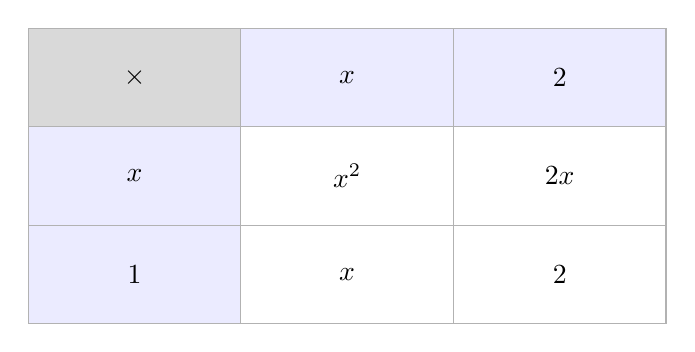
\begin{tikzpicture}[x=1cm,y=1cm]
\fill[gray!30] (0,0) rectangle (2.7,-1.25);
\draw[gray!60] (0,0) rectangle (2.7,-1.25);
\node at (1.35,-0.625) {$\displaystyle \times$};
\fill[blue!8] (2.7,0) rectangle (5.4,-1.25);
\draw[gray!60] (2.7,0) rectangle (5.4,-1.25);
\node at (4.05,-0.625) {$\displaystyle x$};
\fill[blue!8] (5.4,0) rectangle (8.1,-1.25);
\draw[gray!60] (5.4,0) rectangle (8.1,-1.25);
\node at (6.75,-0.625) {$\displaystyle 2$};
\fill[blue!8] (0,-1.25) rectangle (2.7,-2.5);
\draw[gray!60] (0,-1.25) rectangle (2.7,-2.5);
\node at (1.35,-1.875) {$\displaystyle x$};
\fill[white] (2.7,-1.25) rectangle (5.4,-2.5);
\draw[gray!60] (2.7,-1.25) rectangle (5.4,-2.5);
\node at (4.05,-1.875) {$\displaystyle x^2$};
\fill[white] (5.4,-1.25) rectangle (8.1,-2.5);
\draw[gray!60] (5.4,-1.25) rectangle (8.1,-2.5);
\node at (6.75,-1.875) {$\displaystyle 2x$};
\fill[blue!8] (0,-2.5) rectangle (2.7,-3.75);
\draw[gray!60] (0,-2.5) rectangle (2.7,-3.75);
\node at (1.35,-3.125) {$\displaystyle 1$};
\fill[white] (2.7,-2.5) rectangle (5.4,-3.75);
\draw[gray!60] (2.7,-2.5) rectangle (5.4,-3.75);
\node at (4.05,-3.125) {$\displaystyle x$};
\fill[white] (5.4,-2.5) rectangle (8.1,-3.75);
\draw[gray!60] (5.4,-2.5) rectangle (8.1,-3.75);
\node at (6.75,-3.125) {$\displaystyle 2$};
\end{tikzpicture}
\end{center}
\small Grid for $(x+1)(x+2)$; this product is subtracted from $2x(x+3)=2x^2+6x$.\normalsize

\medskip\hrule

\section*{Expanding Brackets 22\quad\small\texttt{(a1-022)}}
\addcontentsline{toc}{section}{Expanding Brackets 22 (a1-022)}
\textit{Difficulty: Foundation \quad\textbar\quad Marks: 4}

\question{Expand and simplify \( (a + b)^2 - (a - b)^2 \).}

\textbf{Worked solution.}

\textit{Expand both squared brackets}
\[\begin{gathered}
\begin{aligned} (a+b)^2 - (a-b)^2 &= (a+b)(a+b)-(a-b)(a-b) \\ &= a(a+b)+b(a+b) - \Big[a(a-b)-b(a-b)\Big] \\ &= a^2+ab+ab+b^2-(a^2-ab-ab+b^2) \\ &= a^2+2ab+b^2-a^2+2ab-b^2 \\ &= 4ab \end{aligned}
\end{gathered}\]
Expand each squared bracket using a(c+d)+b(c+d), then subtract and collect like terms.

\begin{answerbox}
\textbf{Final answer:}\quad \(\displaystyle 4ab\)
\end{answerbox}
\textbf{Area-model diagram.}

\begin{center}
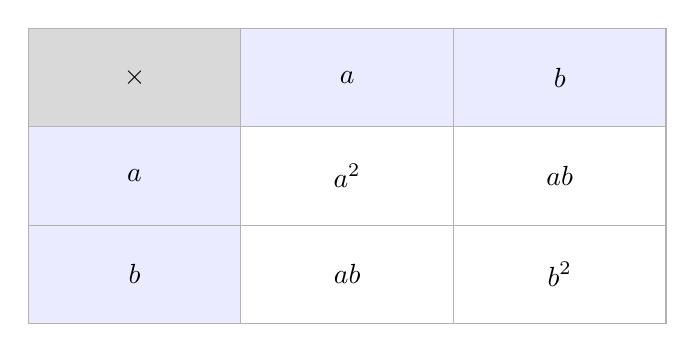
\begin{tikzpicture}[x=1cm,y=1cm]
\fill[gray!30] (0,0) rectangle (2.7,-1.25);
\draw[gray!60] (0,0) rectangle (2.7,-1.25);
\node at (1.35,-0.625) {$\displaystyle \times$};
\fill[blue!8] (2.7,0) rectangle (5.4,-1.25);
\draw[gray!60] (2.7,0) rectangle (5.4,-1.25);
\node at (4.05,-0.625) {$\displaystyle a$};
\fill[blue!8] (5.4,0) rectangle (8.1,-1.25);
\draw[gray!60] (5.4,0) rectangle (8.1,-1.25);
\node at (6.75,-0.625) {$\displaystyle b$};
\fill[blue!8] (0,-1.25) rectangle (2.7,-2.5);
\draw[gray!60] (0,-1.25) rectangle (2.7,-2.5);
\node at (1.35,-1.875) {$\displaystyle a$};
\fill[white] (2.7,-1.25) rectangle (5.4,-2.5);
\draw[gray!60] (2.7,-1.25) rectangle (5.4,-2.5);
\node at (4.05,-1.875) {$\displaystyle a^2$};
\fill[white] (5.4,-1.25) rectangle (8.1,-2.5);
\draw[gray!60] (5.4,-1.25) rectangle (8.1,-2.5);
\node at (6.75,-1.875) {$\displaystyle ab$};
\fill[blue!8] (0,-2.5) rectangle (2.7,-3.75);
\draw[gray!60] (0,-2.5) rectangle (2.7,-3.75);
\node at (1.35,-3.125) {$\displaystyle b$};
\fill[white] (2.7,-2.5) rectangle (5.4,-3.75);
\draw[gray!60] (2.7,-2.5) rectangle (5.4,-3.75);
\node at (4.05,-3.125) {$\displaystyle ab$};
\fill[white] (5.4,-2.5) rectangle (8.1,-3.75);
\draw[gray!60] (5.4,-2.5) rectangle (8.1,-3.75);
\node at (6.75,-3.125) {$\displaystyle b^2$};
\end{tikzpicture}
\end{center}
\small Grid for $(a+b)^2$; subtract the analogous grid for $(a-b)^2$.\normalsize

\medskip\hrule

\section*{Expanding Brackets 23\quad\small\texttt{(a1-023)}}
\addcontentsline{toc}{section}{Expanding Brackets 23 (a1-023)}
\textit{Difficulty: Foundation \quad\textbar\quad Marks: 3}

\question{Expand \( x[3(x + 2) - 4] \).}

\textbf{Worked solution.}

\textit{Simplify the expression inside the square brackets first}
\[\begin{gathered}
\begin{aligned} x(3(x + 2) - 4) &= x(3x+6-4) \\ &= x(3x+2) \\ &= 3x^2+2x \end{aligned}
\end{gathered}\]
Start from the inner-most brackets and work outward.

\begin{answerbox}
\textbf{Final answer:}\quad \(\displaystyle 3x^2 + 2x\)
\end{answerbox}
\textbf{Area-model diagram.}

\begin{center}
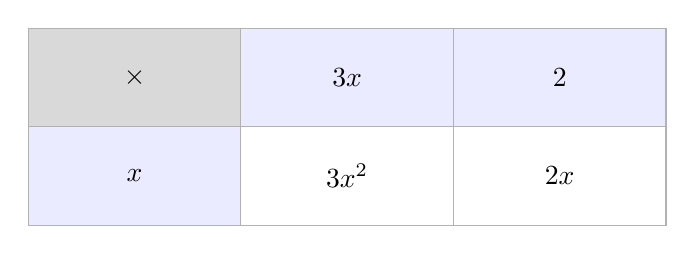
\begin{tikzpicture}[x=1cm,y=1cm]
\fill[gray!30] (0,0) rectangle (2.7,-1.25);
\draw[gray!60] (0,0) rectangle (2.7,-1.25);
\node at (1.35,-0.625) {$\displaystyle \times$};
\fill[blue!8] (2.7,0) rectangle (5.4,-1.25);
\draw[gray!60] (2.7,0) rectangle (5.4,-1.25);
\node at (4.05,-0.625) {$\displaystyle 3x$};
\fill[blue!8] (5.4,0) rectangle (8.1,-1.25);
\draw[gray!60] (5.4,0) rectangle (8.1,-1.25);
\node at (6.75,-0.625) {$\displaystyle 2$};
\fill[blue!8] (0,-1.25) rectangle (2.7,-2.5);
\draw[gray!60] (0,-1.25) rectangle (2.7,-2.5);
\node at (1.35,-1.875) {$\displaystyle x$};
\fill[white] (2.7,-1.25) rectangle (5.4,-2.5);
\draw[gray!60] (2.7,-1.25) rectangle (5.4,-2.5);
\node at (4.05,-1.875) {$\displaystyle 3x^2$};
\fill[white] (5.4,-1.25) rectangle (8.1,-2.5);
\draw[gray!60] (5.4,-1.25) rectangle (8.1,-2.5);
\node at (6.75,-1.875) {$\displaystyle 2x$};
\end{tikzpicture}
\end{center}
\small After simplifying the inside to $(3x+2)$, this grid multiplies by $x$.\normalsize

\medskip\hrule

\section*{Expanding Brackets 24\quad\small\texttt{(a1-024)}}
\addcontentsline{toc}{section}{Expanding Brackets 24 (a1-024)}
\textit{Difficulty: Foundation \quad\textbar\quad Marks: 4}

\question{Expand and simplify \( \left(x + \frac{1}{x^2}\right)\left(y - \frac{1}{z^2}\right) \).}

\textbf{Worked solution.}

\textit{Expand the brackets}
\[\begin{gathered}
\begin{aligned} \left( x + \frac{1}{x^2}\right)\left(y - \frac{1}{z^2}\right) &= x\left(y-\frac{1}{z^2}\right) +\frac{1}{x^2}\left( y - \frac{1}{z^2}\right) \\ &= xy - \frac{x}{z^2} + \frac{y}{x^2} - \frac{1}{x^2z^2} \end{aligned}
\end{gathered}\]
Multiply each term in the first bracket by each term in the second. Since all variables are different, no terms can be combined.

\begin{answerbox}
\textbf{Final answer:}\quad \(\displaystyle xy - \frac{x}{z^2} + \frac{y}{x^2} - \frac{1}{x^2z^2}\)
\end{answerbox}
\textbf{Area-model diagram.}

\begin{center}
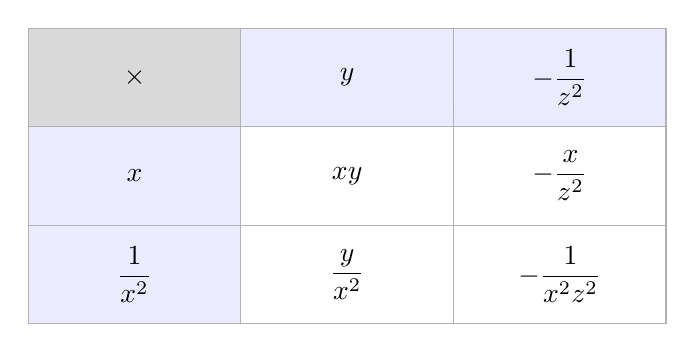
\begin{tikzpicture}[x=1cm,y=1cm]
\fill[gray!30] (0,0) rectangle (2.7,-1.25);
\draw[gray!60] (0,0) rectangle (2.7,-1.25);
\node at (1.35,-0.625) {$\displaystyle \times$};
\fill[blue!8] (2.7,0) rectangle (5.4,-1.25);
\draw[gray!60] (2.7,0) rectangle (5.4,-1.25);
\node at (4.05,-0.625) {$\displaystyle y$};
\fill[blue!8] (5.4,0) rectangle (8.1,-1.25);
\draw[gray!60] (5.4,0) rectangle (8.1,-1.25);
\node at (6.75,-0.625) {$\displaystyle -\frac{1}{z^2}$};
\fill[blue!8] (0,-1.25) rectangle (2.7,-2.5);
\draw[gray!60] (0,-1.25) rectangle (2.7,-2.5);
\node at (1.35,-1.875) {$\displaystyle x$};
\fill[white] (2.7,-1.25) rectangle (5.4,-2.5);
\draw[gray!60] (2.7,-1.25) rectangle (5.4,-2.5);
\node at (4.05,-1.875) {$\displaystyle xy$};
\fill[white] (5.4,-1.25) rectangle (8.1,-2.5);
\draw[gray!60] (5.4,-1.25) rectangle (8.1,-2.5);
\node at (6.75,-1.875) {$\displaystyle -\frac{x}{z^2}$};
\fill[blue!8] (0,-2.5) rectangle (2.7,-3.75);
\draw[gray!60] (0,-2.5) rectangle (2.7,-3.75);
\node at (1.35,-3.125) {$\displaystyle \frac{1}{x^2}$};
\fill[white] (2.7,-2.5) rectangle (5.4,-3.75);
\draw[gray!60] (2.7,-2.5) rectangle (5.4,-3.75);
\node at (4.05,-3.125) {$\displaystyle \frac{y}{x^2}$};
\fill[white] (5.4,-2.5) rectangle (8.1,-3.75);
\draw[gray!60] (5.4,-2.5) rectangle (8.1,-3.75);
\node at (6.75,-3.125) {$\displaystyle -\frac{1}{x^2z^2}$};
\end{tikzpicture}
\end{center}
\medskip\hrule

\section*{Expanding Brackets 25\quad\small\texttt{(a1-025)}}
\addcontentsline{toc}{section}{Expanding Brackets 25 (a1-025)}
\textit{Difficulty: Foundation \quad\textbar\quad Marks: 3}

\question{Expand and simplify \( (a + b)(a^2 - b^2) \).}

\textbf{Worked solution.}

\textit{Expand the brackets}
\[\begin{gathered}
\begin{aligned} (a+b)(a^2-b^2) &= a(a^2-b^2) + b(a^2-b^2) \\ &= a^3 - ab^2 + a^2b - b^3 \\ &= a^3 + a^2b - ab^2 - b^3 \end{aligned}
\end{gathered}\]
Distribute the \(a\) and the \(b\) across the second bracket. Remember to add the indices for the same bases (\(a \times a^2 = a^3\)).

\begin{answerbox}
\textbf{Final answer:}\quad \(\displaystyle a^3 + a^2b - ab^2 - b^3\)
\end{answerbox}
\textbf{Area-model diagram.}

\begin{center}
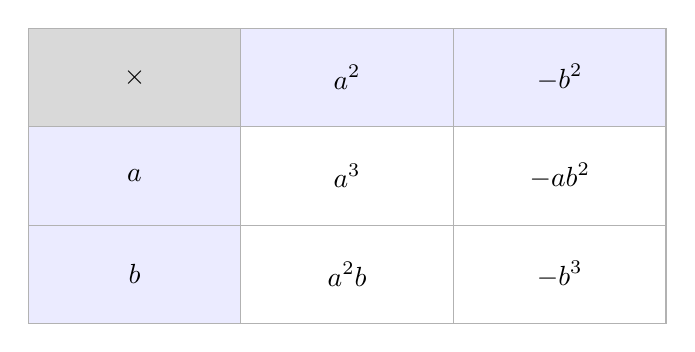
\begin{tikzpicture}[x=1cm,y=1cm]
\fill[gray!30] (0,0) rectangle (2.7,-1.25);
\draw[gray!60] (0,0) rectangle (2.7,-1.25);
\node at (1.35,-0.625) {$\displaystyle \times$};
\fill[blue!8] (2.7,0) rectangle (5.4,-1.25);
\draw[gray!60] (2.7,0) rectangle (5.4,-1.25);
\node at (4.05,-0.625) {$\displaystyle a^2$};
\fill[blue!8] (5.4,0) rectangle (8.1,-1.25);
\draw[gray!60] (5.4,0) rectangle (8.1,-1.25);
\node at (6.75,-0.625) {$\displaystyle -b^2$};
\fill[blue!8] (0,-1.25) rectangle (2.7,-2.5);
\draw[gray!60] (0,-1.25) rectangle (2.7,-2.5);
\node at (1.35,-1.875) {$\displaystyle a$};
\fill[white] (2.7,-1.25) rectangle (5.4,-2.5);
\draw[gray!60] (2.7,-1.25) rectangle (5.4,-2.5);
\node at (4.05,-1.875) {$\displaystyle a^3$};
\fill[white] (5.4,-1.25) rectangle (8.1,-2.5);
\draw[gray!60] (5.4,-1.25) rectangle (8.1,-2.5);
\node at (6.75,-1.875) {$\displaystyle -ab^2$};
\fill[blue!8] (0,-2.5) rectangle (2.7,-3.75);
\draw[gray!60] (0,-2.5) rectangle (2.7,-3.75);
\node at (1.35,-3.125) {$\displaystyle b$};
\fill[white] (2.7,-2.5) rectangle (5.4,-3.75);
\draw[gray!60] (2.7,-2.5) rectangle (5.4,-3.75);
\node at (4.05,-3.125) {$\displaystyle a^2b$};
\fill[white] (5.4,-2.5) rectangle (8.1,-3.75);
\draw[gray!60] (5.4,-2.5) rectangle (8.1,-3.75);
\node at (6.75,-3.125) {$\displaystyle -b^3$};
\end{tikzpicture}
\end{center}
\medskip\hrule

\section*{Expanding Brackets 26\quad\small\texttt{(a1-026)}}
\addcontentsline{toc}{section}{Expanding Brackets 26 (a1-026)}
\textit{Difficulty: Foundation \quad\textbar\quad Marks: 4}

\question{Expand and simplify \( p(p + q) - pq(p^2 - pq) \).}

\textbf{Worked solution.}

\textit{Expand each part of the expression}
\[\begin{gathered}
\begin{aligned} p(p + q) - pq(p^2-pq) &= p(p) + p(q) - pq(p^2) - pq(-pq) \\ &= p^2 + pq - p^3q + p^2q^2 \end{aligned}
\end{gathered}\]
Be careful with the second part; multiplying \(-pq\) by \(-pq\) results in a positive \(+p^2q^2\).

\begin{answerbox}
\textbf{Final answer:}\quad \(\displaystyle p^2 + pq - p^3q + p^2q^2\)
\end{answerbox}
\textbf{Area-model diagram.}

\begin{center}
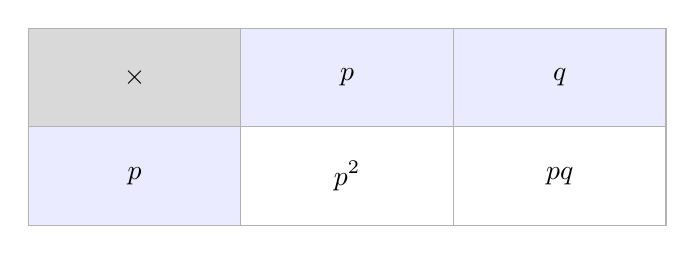
\begin{tikzpicture}[x=1cm,y=1cm]
\fill[gray!30] (0,0) rectangle (2.7,-1.25);
\draw[gray!60] (0,0) rectangle (2.7,-1.25);
\node at (1.35,-0.625) {$\displaystyle \times$};
\fill[blue!8] (2.7,0) rectangle (5.4,-1.25);
\draw[gray!60] (2.7,0) rectangle (5.4,-1.25);
\node at (4.05,-0.625) {$\displaystyle p$};
\fill[blue!8] (5.4,0) rectangle (8.1,-1.25);
\draw[gray!60] (5.4,0) rectangle (8.1,-1.25);
\node at (6.75,-0.625) {$\displaystyle q$};
\fill[blue!8] (0,-1.25) rectangle (2.7,-2.5);
\draw[gray!60] (0,-1.25) rectangle (2.7,-2.5);
\node at (1.35,-1.875) {$\displaystyle p$};
\fill[white] (2.7,-1.25) rectangle (5.4,-2.5);
\draw[gray!60] (2.7,-1.25) rectangle (5.4,-2.5);
\node at (4.05,-1.875) {$\displaystyle p^2$};
\fill[white] (5.4,-1.25) rectangle (8.1,-2.5);
\draw[gray!60] (5.4,-1.25) rectangle (8.1,-2.5);
\node at (6.75,-1.875) {$\displaystyle pq$};
\end{tikzpicture}
\end{center}
\small Grid for $p(p+q)$; from this subtract $pq(p^2-pq)=p^3q-p^2q^2$.\normalsize

\medskip\hrule

\section*{Expanding Brackets 27\quad\small\texttt{(a1-027)}}
\addcontentsline{toc}{section}{Expanding Brackets 27 (a1-027)}
\textit{Difficulty: Foundation \quad\textbar\quad Marks: 4}

\question{Expand and simplify \( \left(\frac{3}{x} - \frac{4}{x^2}\right)(x^2 + 3x) \).}

\textbf{Worked solution.}

\textit{Distribute the fractional terms}
\[\begin{gathered}
\begin{aligned} \left(\frac{3}{x} - \frac{4}{x^2}\right)\left(x^2+3x\right) &= \frac{3}{x}(x^2+3x)-\frac{4}{x^2}(x^2+3x) \\ &= 3x+9-4-\frac{12}{x} \\ &= 3x+5-\frac{12}{x} \end{aligned}
\end{gathered}\]
Multiply each term in the first bracket by each term in the second.

\begin{answerbox}
\textbf{Final answer:}\quad \(\displaystyle 3x + 5 - \frac{12}{x}\)
\end{answerbox}
\textbf{Area-model diagram.}

\begin{center}
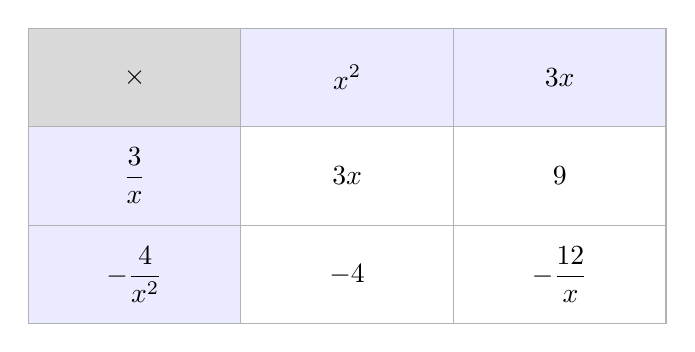
\begin{tikzpicture}[x=1cm,y=1cm]
\fill[gray!30] (0,0) rectangle (2.7,-1.25);
\draw[gray!60] (0,0) rectangle (2.7,-1.25);
\node at (1.35,-0.625) {$\displaystyle \times$};
\fill[blue!8] (2.7,0) rectangle (5.4,-1.25);
\draw[gray!60] (2.7,0) rectangle (5.4,-1.25);
\node at (4.05,-0.625) {$\displaystyle x^2$};
\fill[blue!8] (5.4,0) rectangle (8.1,-1.25);
\draw[gray!60] (5.4,0) rectangle (8.1,-1.25);
\node at (6.75,-0.625) {$\displaystyle 3x$};
\fill[blue!8] (0,-1.25) rectangle (2.7,-2.5);
\draw[gray!60] (0,-1.25) rectangle (2.7,-2.5);
\node at (1.35,-1.875) {$\displaystyle \frac{3}{x}$};
\fill[white] (2.7,-1.25) rectangle (5.4,-2.5);
\draw[gray!60] (2.7,-1.25) rectangle (5.4,-2.5);
\node at (4.05,-1.875) {$\displaystyle 3x$};
\fill[white] (5.4,-1.25) rectangle (8.1,-2.5);
\draw[gray!60] (5.4,-1.25) rectangle (8.1,-2.5);
\node at (6.75,-1.875) {$\displaystyle 9$};
\fill[blue!8] (0,-2.5) rectangle (2.7,-3.75);
\draw[gray!60] (0,-2.5) rectangle (2.7,-3.75);
\node at (1.35,-3.125) {$\displaystyle -\frac{4}{x^2}$};
\fill[white] (2.7,-2.5) rectangle (5.4,-3.75);
\draw[gray!60] (2.7,-2.5) rectangle (5.4,-3.75);
\node at (4.05,-3.125) {$\displaystyle -4$};
\fill[white] (5.4,-2.5) rectangle (8.1,-3.75);
\draw[gray!60] (5.4,-2.5) rectangle (8.1,-3.75);
\node at (6.75,-3.125) {$\displaystyle -\frac{12}{x}$};
\end{tikzpicture}
\end{center}
\medskip\hrule

\section*{Expanding Brackets 28\quad\small\texttt{(a1-028)}}
\addcontentsline{toc}{section}{Expanding Brackets 28 (a1-028)}
\textit{Difficulty: Foundation \quad\textbar\quad Marks: 3}

\question{Expand and simplify \( (x^2 - 1)\left(1 + \frac{1}{x}\right) \).}

\textbf{Worked solution.}

\textit{Expand the brackets}
\[\begin{gathered}
\begin{aligned} (x^2-1)\left( 1 +\frac{1}{x}\right) &= x^2\left( 1 +\frac{1}{x}\right) -1\left( 1 +\frac{1}{x}\right) \\ &= x^2 + x - 1 - \frac{1}{x} \end{aligned}
\end{gathered}\]
Multiply through and simplify \(x^2 \times \frac{1}{x}\) to get \(x\).

\begin{answerbox}
\textbf{Final answer:}\quad \(\displaystyle x^2 + x - 1 - \frac{1}{x}\)
\end{answerbox}
\textbf{Area-model diagram.}

\begin{center}
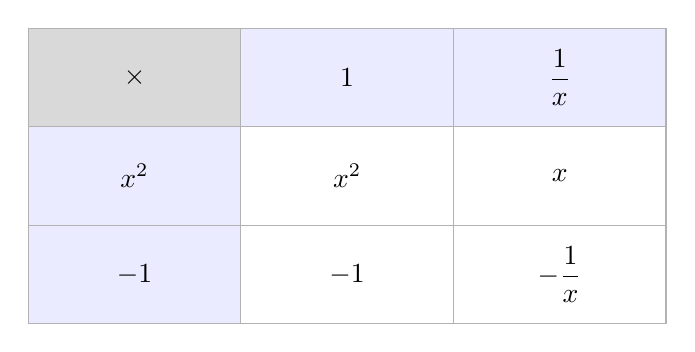
\begin{tikzpicture}[x=1cm,y=1cm]
\fill[gray!30] (0,0) rectangle (2.7,-1.25);
\draw[gray!60] (0,0) rectangle (2.7,-1.25);
\node at (1.35,-0.625) {$\displaystyle \times$};
\fill[blue!8] (2.7,0) rectangle (5.4,-1.25);
\draw[gray!60] (2.7,0) rectangle (5.4,-1.25);
\node at (4.05,-0.625) {$\displaystyle 1$};
\fill[blue!8] (5.4,0) rectangle (8.1,-1.25);
\draw[gray!60] (5.4,0) rectangle (8.1,-1.25);
\node at (6.75,-0.625) {$\displaystyle \frac{1}{x}$};
\fill[blue!8] (0,-1.25) rectangle (2.7,-2.5);
\draw[gray!60] (0,-1.25) rectangle (2.7,-2.5);
\node at (1.35,-1.875) {$\displaystyle x^2$};
\fill[white] (2.7,-1.25) rectangle (5.4,-2.5);
\draw[gray!60] (2.7,-1.25) rectangle (5.4,-2.5);
\node at (4.05,-1.875) {$\displaystyle x^2$};
\fill[white] (5.4,-1.25) rectangle (8.1,-2.5);
\draw[gray!60] (5.4,-1.25) rectangle (8.1,-2.5);
\node at (6.75,-1.875) {$\displaystyle x$};
\fill[blue!8] (0,-2.5) rectangle (2.7,-3.75);
\draw[gray!60] (0,-2.5) rectangle (2.7,-3.75);
\node at (1.35,-3.125) {$\displaystyle -1$};
\fill[white] (2.7,-2.5) rectangle (5.4,-3.75);
\draw[gray!60] (2.7,-2.5) rectangle (5.4,-3.75);
\node at (4.05,-3.125) {$\displaystyle -1$};
\fill[white] (5.4,-2.5) rectangle (8.1,-3.75);
\draw[gray!60] (5.4,-2.5) rectangle (8.1,-3.75);
\node at (6.75,-3.125) {$\displaystyle -\frac{1}{x}$};
\end{tikzpicture}
\end{center}
\medskip\hrule

\section*{Expanding Brackets 29\quad\small\texttt{(a1-029)}}
\addcontentsline{toc}{section}{Expanding Brackets 29 (a1-029)}
\textit{Difficulty: Foundation \quad\textbar\quad Marks: 4}

\question{Expand and simplify \( \left(y^2 + \frac{1}{y}\right)(y^3 - 2) \).}

\textbf{Worked solution.}

\textit{Expand the brackets and simplify the powers}
\[\begin{gathered}
\begin{aligned} \left(y^2 + \frac{1}{y}\right)(y^3 - 2) &= y^2(y^3 - 2) + \frac{1}{y}(y^3 - 2) \\ &= y^5 - 2y^2 + \frac{y^3}{y} - \frac{2}{y} \\ &= y^5 - 2y^2 + y^2 - \frac{2}{y} \\ &= y^5 - y^2 - \frac{2}{y} \end{aligned}
\end{gathered}\]
Multiply both terms in the first bracket by both terms in the second. Simplify \( \frac{y^3}{y} \) to \( y^2 \) using index laws.

\begin{answerbox}
\textbf{Final answer:}\quad \(\displaystyle y^5 - y^2 - \frac{2}{y}\)
\end{answerbox}
\textbf{Area-model diagram.}

\begin{center}
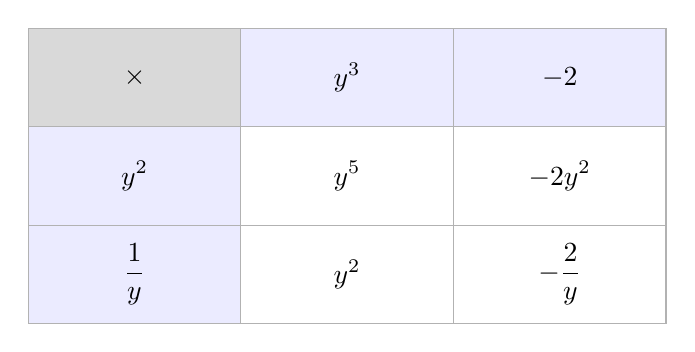
\begin{tikzpicture}[x=1cm,y=1cm]
\fill[gray!30] (0,0) rectangle (2.7,-1.25);
\draw[gray!60] (0,0) rectangle (2.7,-1.25);
\node at (1.35,-0.625) {$\displaystyle \times$};
\fill[blue!8] (2.7,0) rectangle (5.4,-1.25);
\draw[gray!60] (2.7,0) rectangle (5.4,-1.25);
\node at (4.05,-0.625) {$\displaystyle y^3$};
\fill[blue!8] (5.4,0) rectangle (8.1,-1.25);
\draw[gray!60] (5.4,0) rectangle (8.1,-1.25);
\node at (6.75,-0.625) {$\displaystyle -2$};
\fill[blue!8] (0,-1.25) rectangle (2.7,-2.5);
\draw[gray!60] (0,-1.25) rectangle (2.7,-2.5);
\node at (1.35,-1.875) {$\displaystyle y^2$};
\fill[white] (2.7,-1.25) rectangle (5.4,-2.5);
\draw[gray!60] (2.7,-1.25) rectangle (5.4,-2.5);
\node at (4.05,-1.875) {$\displaystyle y^5$};
\fill[white] (5.4,-1.25) rectangle (8.1,-2.5);
\draw[gray!60] (5.4,-1.25) rectangle (8.1,-2.5);
\node at (6.75,-1.875) {$\displaystyle -2y^2$};
\fill[blue!8] (0,-2.5) rectangle (2.7,-3.75);
\draw[gray!60] (0,-2.5) rectangle (2.7,-3.75);
\node at (1.35,-3.125) {$\displaystyle \frac{1}{y}$};
\fill[white] (2.7,-2.5) rectangle (5.4,-3.75);
\draw[gray!60] (2.7,-2.5) rectangle (5.4,-3.75);
\node at (4.05,-3.125) {$\displaystyle y^2$};
\fill[white] (5.4,-2.5) rectangle (8.1,-3.75);
\draw[gray!60] (5.4,-2.5) rectangle (8.1,-3.75);
\node at (6.75,-3.125) {$\displaystyle -\frac{2}{y}$};
\end{tikzpicture}
\end{center}
\medskip\hrule

\section*{Expanding Brackets 30\quad\small\texttt{(a1-030)}}
\addcontentsline{toc}{section}{Expanding Brackets 30 (a1-030)}
\textit{Difficulty: Foundation \quad\textbar\quad Marks: 3}

\question{Expand and simplify \( 2ab(a - b) - a^2(2b - 1) \).}

\textbf{Worked solution.}

\textit{Expand and simplify}
\[\begin{gathered}
\begin{aligned} 2ab(a - b) - a^2(2b - 1) &= 2a^2b - 2ab^2 - 2a^2b + a^2 \\ &= a^2 - 2ab^2 \end{aligned}
\end{gathered}\]
Distribute each term, then the \(2a^2b\) and \(-2a^2b\) cancel, leaving \(a^2 - 2ab^2\).

\begin{answerbox}
\textbf{Final answer:}\quad \(\displaystyle a^2 - 2ab^2\)
\end{answerbox}
\textbf{Area-model diagram.}

\begin{center}
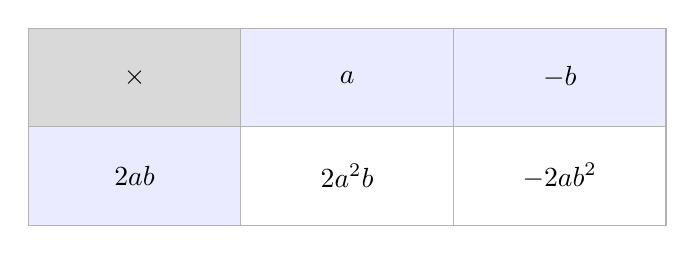
\begin{tikzpicture}[x=1cm,y=1cm]
\fill[gray!30] (0,0) rectangle (2.7,-1.25);
\draw[gray!60] (0,0) rectangle (2.7,-1.25);
\node at (1.35,-0.625) {$\displaystyle \times$};
\fill[blue!8] (2.7,0) rectangle (5.4,-1.25);
\draw[gray!60] (2.7,0) rectangle (5.4,-1.25);
\node at (4.05,-0.625) {$\displaystyle a$};
\fill[blue!8] (5.4,0) rectangle (8.1,-1.25);
\draw[gray!60] (5.4,0) rectangle (8.1,-1.25);
\node at (6.75,-0.625) {$\displaystyle -b$};
\fill[blue!8] (0,-1.25) rectangle (2.7,-2.5);
\draw[gray!60] (0,-1.25) rectangle (2.7,-2.5);
\node at (1.35,-1.875) {$\displaystyle 2ab$};
\fill[white] (2.7,-1.25) rectangle (5.4,-2.5);
\draw[gray!60] (2.7,-1.25) rectangle (5.4,-2.5);
\node at (4.05,-1.875) {$\displaystyle 2a^2b$};
\fill[white] (5.4,-1.25) rectangle (8.1,-2.5);
\draw[gray!60] (5.4,-1.25) rectangle (8.1,-2.5);
\node at (6.75,-1.875) {$\displaystyle -2ab^2$};
\end{tikzpicture}
\end{center}
\small Grid for $2ab(a-b)$; from this subtract $a^2(2b-1)=2a^2b-a^2$.\normalsize

\medskip\hrule

\section*{Expanding Brackets 31\quad\small\texttt{(a1-031)}}
\addcontentsline{toc}{section}{Expanding Brackets 31 (a1-031)}
\textit{Difficulty: Foundation \quad\textbar\quad Marks: 4}

\question{Expand and simplify \( \left(\frac{x}{2} + 4\right)\left(\frac{4}{x} - 2\right) \).}

\textbf{Worked solution.}

\textit{Expand and simplify}
\[\begin{gathered}
\begin{aligned} \left(\frac{x}{2} + 4\right)\left(\frac{4}{x} - 2\right) &= \frac{x}{2}\left(\frac{4}{x} - 2\right) + 4\left(\frac{4}{x} - 2\right) \\ &= \frac{4x}{2x} - \frac{2x}{2} + \frac{16}{x} - 8 \\ &= 2 - x + \frac{16}{x} - 8 \\ &= \frac{16}{x} - x - 6 \end{aligned}
\end{gathered}\]
Distribute each term in the first bracket across the second bracket, simplify the fractions, then collect like terms.

\begin{answerbox}
\textbf{Final answer:}\quad \(\displaystyle \frac{16}{x} - x - 6\)
\end{answerbox}
\textbf{Area-model diagram.}

\begin{center}
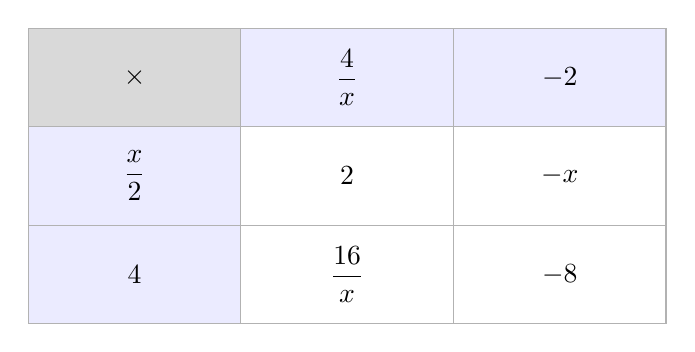
\begin{tikzpicture}[x=1cm,y=1cm]
\fill[gray!30] (0,0) rectangle (2.7,-1.25);
\draw[gray!60] (0,0) rectangle (2.7,-1.25);
\node at (1.35,-0.625) {$\displaystyle \times$};
\fill[blue!8] (2.7,0) rectangle (5.4,-1.25);
\draw[gray!60] (2.7,0) rectangle (5.4,-1.25);
\node at (4.05,-0.625) {$\displaystyle \frac{4}{x}$};
\fill[blue!8] (5.4,0) rectangle (8.1,-1.25);
\draw[gray!60] (5.4,0) rectangle (8.1,-1.25);
\node at (6.75,-0.625) {$\displaystyle -2$};
\fill[blue!8] (0,-1.25) rectangle (2.7,-2.5);
\draw[gray!60] (0,-1.25) rectangle (2.7,-2.5);
\node at (1.35,-1.875) {$\displaystyle \frac{x}{2}$};
\fill[white] (2.7,-1.25) rectangle (5.4,-2.5);
\draw[gray!60] (2.7,-1.25) rectangle (5.4,-2.5);
\node at (4.05,-1.875) {$\displaystyle 2$};
\fill[white] (5.4,-1.25) rectangle (8.1,-2.5);
\draw[gray!60] (5.4,-1.25) rectangle (8.1,-2.5);
\node at (6.75,-1.875) {$\displaystyle -x$};
\fill[blue!8] (0,-2.5) rectangle (2.7,-3.75);
\draw[gray!60] (0,-2.5) rectangle (2.7,-3.75);
\node at (1.35,-3.125) {$\displaystyle 4$};
\fill[white] (2.7,-2.5) rectangle (5.4,-3.75);
\draw[gray!60] (2.7,-2.5) rectangle (5.4,-3.75);
\node at (4.05,-3.125) {$\displaystyle \frac{16}{x}$};
\fill[white] (5.4,-2.5) rectangle (8.1,-3.75);
\draw[gray!60] (5.4,-2.5) rectangle (8.1,-3.75);
\node at (6.75,-3.125) {$\displaystyle -8$};
\end{tikzpicture}
\end{center}
\medskip\hrule

\section*{Expanding Brackets 32\quad\small\texttt{(a1-032)}}
\addcontentsline{toc}{section}{Expanding Brackets 32 (a1-032)}
\textit{Difficulty: Foundation \quad\textbar\quad Marks: 3}

\question{Expand and simplify \( m^2n(m + n) - n^2m(n + m) \).}

\textbf{Worked solution.}

\textit{Expand and simplify}
\[\begin{gathered}
\begin{aligned} m^2n(m + n) - n^2m(n + m) &= m^3n + m^2n^2 - n^3m - n^2m^2 \\ &= m^3n - mn^3 \end{aligned}
\end{gathered}\]
Distribute each term, then \(m^2n^2\) and \(-n^2m^2\) cancel, leaving \(m^3n - mn^3\).

\begin{answerbox}
\textbf{Final answer:}\quad \(\displaystyle m^3n - mn^3\)
\end{answerbox}
\textbf{Area-model diagram.}

\begin{center}
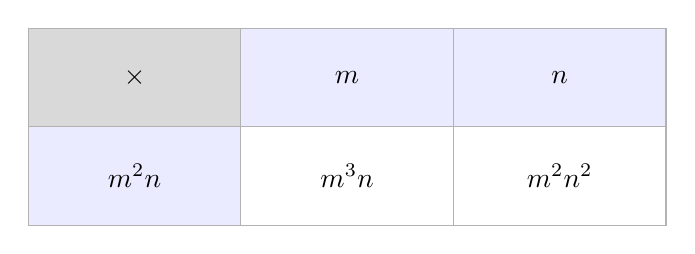
\begin{tikzpicture}[x=1cm,y=1cm]
\fill[gray!30] (0,0) rectangle (2.7,-1.25);
\draw[gray!60] (0,0) rectangle (2.7,-1.25);
\node at (1.35,-0.625) {$\displaystyle \times$};
\fill[blue!8] (2.7,0) rectangle (5.4,-1.25);
\draw[gray!60] (2.7,0) rectangle (5.4,-1.25);
\node at (4.05,-0.625) {$\displaystyle m$};
\fill[blue!8] (5.4,0) rectangle (8.1,-1.25);
\draw[gray!60] (5.4,0) rectangle (8.1,-1.25);
\node at (6.75,-0.625) {$\displaystyle n$};
\fill[blue!8] (0,-1.25) rectangle (2.7,-2.5);
\draw[gray!60] (0,-1.25) rectangle (2.7,-2.5);
\node at (1.35,-1.875) {$\displaystyle m^2n$};
\fill[white] (2.7,-1.25) rectangle (5.4,-2.5);
\draw[gray!60] (2.7,-1.25) rectangle (5.4,-2.5);
\node at (4.05,-1.875) {$\displaystyle m^3n$};
\fill[white] (5.4,-1.25) rectangle (8.1,-2.5);
\draw[gray!60] (5.4,-1.25) rectangle (8.1,-2.5);
\node at (6.75,-1.875) {$\displaystyle m^2n^2$};
\end{tikzpicture}
\end{center}
\small Grid for $m^2n(m+n)$; from this subtract $n^2m(n+m)=mn^3+m^2n^2$.\normalsize

\medskip\hrule

\section*{Expanding Brackets 33\quad\small\texttt{(a1-033)}}
\addcontentsline{toc}{section}{Expanding Brackets 33 (a1-033)}
\textit{Difficulty: Foundation \quad\textbar\quad Marks: 3}

\question{Expand and simplify \( \left(1 - \frac{2}{x}\right)\left(x^2 + 2x\right) \).}

\textbf{Worked solution.}

\textit{Expand and simplify}
\[\begin{gathered}
\begin{aligned} \left(1 - \frac{2}{x}\right)(x^2 + 2x) &= 1(x^2 + 2x) - \frac{2}{x}(x^2 + 2x) \\ &= x^2 + 2x - 2x - 4 \\ &= x^2 - 4 \end{aligned}
\end{gathered}\]
Distribute each term. The \(2x\) terms cancel, leaving \(x^2 - 4\).

\begin{answerbox}
\textbf{Final answer:}\quad \(\displaystyle x^2 - 4\)
\end{answerbox}
\textbf{Area-model diagram.}

\begin{center}
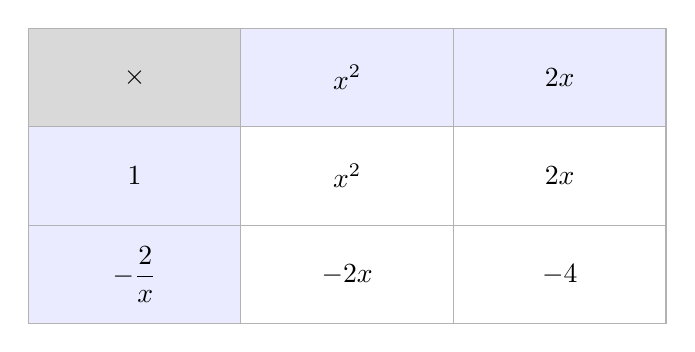
\begin{tikzpicture}[x=1cm,y=1cm]
\fill[gray!30] (0,0) rectangle (2.7,-1.25);
\draw[gray!60] (0,0) rectangle (2.7,-1.25);
\node at (1.35,-0.625) {$\displaystyle \times$};
\fill[blue!8] (2.7,0) rectangle (5.4,-1.25);
\draw[gray!60] (2.7,0) rectangle (5.4,-1.25);
\node at (4.05,-0.625) {$\displaystyle x^2$};
\fill[blue!8] (5.4,0) rectangle (8.1,-1.25);
\draw[gray!60] (5.4,0) rectangle (8.1,-1.25);
\node at (6.75,-0.625) {$\displaystyle 2x$};
\fill[blue!8] (0,-1.25) rectangle (2.7,-2.5);
\draw[gray!60] (0,-1.25) rectangle (2.7,-2.5);
\node at (1.35,-1.875) {$\displaystyle 1$};
\fill[white] (2.7,-1.25) rectangle (5.4,-2.5);
\draw[gray!60] (2.7,-1.25) rectangle (5.4,-2.5);
\node at (4.05,-1.875) {$\displaystyle x^2$};
\fill[white] (5.4,-1.25) rectangle (8.1,-2.5);
\draw[gray!60] (5.4,-1.25) rectangle (8.1,-2.5);
\node at (6.75,-1.875) {$\displaystyle 2x$};
\fill[blue!8] (0,-2.5) rectangle (2.7,-3.75);
\draw[gray!60] (0,-2.5) rectangle (2.7,-3.75);
\node at (1.35,-3.125) {$\displaystyle -\frac{2}{x}$};
\fill[white] (2.7,-2.5) rectangle (5.4,-3.75);
\draw[gray!60] (2.7,-2.5) rectangle (5.4,-3.75);
\node at (4.05,-3.125) {$\displaystyle -2x$};
\fill[white] (5.4,-2.5) rectangle (8.1,-3.75);
\draw[gray!60] (5.4,-2.5) rectangle (8.1,-3.75);
\node at (6.75,-3.125) {$\displaystyle -4$};
\end{tikzpicture}
\end{center}
\medskip\hrule

\section*{Expanding Brackets 34\quad\small\texttt{(a1-034)}}
\addcontentsline{toc}{section}{Expanding Brackets 34 (a1-034)}
\textit{Difficulty: Foundation \quad\textbar\quad Marks: 3}

\question{Expand and simplify \( \left(xyz - \frac{y^2}{xz}\right)\left(x^2z^2 + \frac{x}{yz} \right) \).}

\textbf{Worked solution.}

\textit{Expand the brackets}
\[\begin{gathered}
\begin{aligned} \left(xyz - \frac{y^2}{xz}\right)\left(x^2z^2 + \frac{x}{yz} \right) &= xyz\left(x^2z^2 + \frac{x}{yz}\right) - \frac{y^2}{xz}\left(x^2z^2 + \frac{x}{yz}\right) \\ &= x^3yz^3 + \frac{x^2yz}{yz} - \frac{x^2y^2z^2}{xz} - \frac{xy^2}{xyz^2} \\ &= x^3yz^3 + x^2 - xy^2z - \frac{y}{z^2} \end{aligned}
\end{gathered}\]
Distribute each term. Simplify the second part by dividing each term by \( x \).

\begin{answerbox}
\textbf{Final answer:}\quad \(\displaystyle x^3yz^3 + x^2 - xy^2z - \frac{y}{z^2}\)
\end{answerbox}
\textbf{Area-model diagram.}

\begin{center}
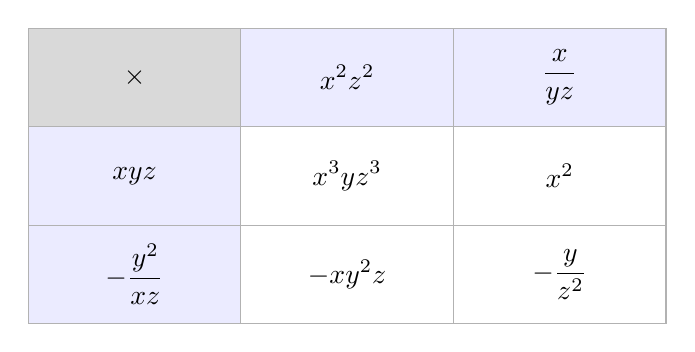
\begin{tikzpicture}[x=1cm,y=1cm]
\fill[gray!30] (0,0) rectangle (2.7,-1.25);
\draw[gray!60] (0,0) rectangle (2.7,-1.25);
\node at (1.35,-0.625) {$\displaystyle \times$};
\fill[blue!8] (2.7,0) rectangle (5.4,-1.25);
\draw[gray!60] (2.7,0) rectangle (5.4,-1.25);
\node at (4.05,-0.625) {$\displaystyle x^2z^2$};
\fill[blue!8] (5.4,0) rectangle (8.1,-1.25);
\draw[gray!60] (5.4,0) rectangle (8.1,-1.25);
\node at (6.75,-0.625) {$\displaystyle \frac{x}{yz}$};
\fill[blue!8] (0,-1.25) rectangle (2.7,-2.5);
\draw[gray!60] (0,-1.25) rectangle (2.7,-2.5);
\node at (1.35,-1.875) {$\displaystyle xyz$};
\fill[white] (2.7,-1.25) rectangle (5.4,-2.5);
\draw[gray!60] (2.7,-1.25) rectangle (5.4,-2.5);
\node at (4.05,-1.875) {$\displaystyle x^3yz^3$};
\fill[white] (5.4,-1.25) rectangle (8.1,-2.5);
\draw[gray!60] (5.4,-1.25) rectangle (8.1,-2.5);
\node at (6.75,-1.875) {$\displaystyle x^2$};
\fill[blue!8] (0,-2.5) rectangle (2.7,-3.75);
\draw[gray!60] (0,-2.5) rectangle (2.7,-3.75);
\node at (1.35,-3.125) {$\displaystyle -\frac{y^2}{xz}$};
\fill[white] (2.7,-2.5) rectangle (5.4,-3.75);
\draw[gray!60] (2.7,-2.5) rectangle (5.4,-3.75);
\node at (4.05,-3.125) {$\displaystyle -xy^2z$};
\fill[white] (5.4,-2.5) rectangle (8.1,-3.75);
\draw[gray!60] (5.4,-2.5) rectangle (8.1,-3.75);
\node at (6.75,-3.125) {$\displaystyle -\frac{y}{z^2}$};
\end{tikzpicture}
\end{center}
\medskip\hrule

\section*{Expanding Brackets 35\quad\small\texttt{(a1-035)}}
\addcontentsline{toc}{section}{Expanding Brackets 35 (a1-035)}
\textit{Difficulty: Foundation \quad\textbar\quad Marks: 4}

\question{Expand and simplify \( \left( x - \frac{1}{x} \right)\left( x^2 + 1 + \frac{1}{x^2} \right)\left( x^3 + \frac{1}{x} \right) \).}

\textbf{Worked solution.}

\textit{Expand the first two brackets, then multiply by the third}
\[\begin{gathered}
\begin{aligned} &\left( x - \frac{1}{x} \right)\left( x^2 + 1 + \frac{1}{x^2} \right)\left( x^3 + \frac{1}{x} \right) \\ &= \left[ x\left( x^2+1+\frac{1}{x^2} \right) -\frac{1}{x}\left( x^2+1+\frac{1}{x^2} \right) \right]\left( x^3 + \frac{1}{x} \right) \\ &= \left[ x^3 + x + \frac{1}{x} - x - \frac{1}{x} - \frac{1}{x^3} \right]\left( x^3 + \frac{1}{x} \right) \\ &= \left( x^3 - \frac{1}{x^3} \right)\left( x^3 + \frac{1}{x} \right) \\ &= x^3\left( x^3 + \frac{1}{x}\right) -\frac{1}{x^3}\left( x^3 + \frac{1}{x} \right) \\ &= x^6 + x^2 - 1 - \frac{1}{x^4} \end{aligned}
\end{gathered}\]
Expand the first two brackets — the middle terms cancel giving a difference of cubes. Then multiply the result by the third bracket.

\begin{answerbox}
\textbf{Final answer:}\quad \(\displaystyle x^6 + x^2 - 1 - \frac{1}{x^4}\)
\end{answerbox}
\textbf{Area-model diagram.}

\begin{center}
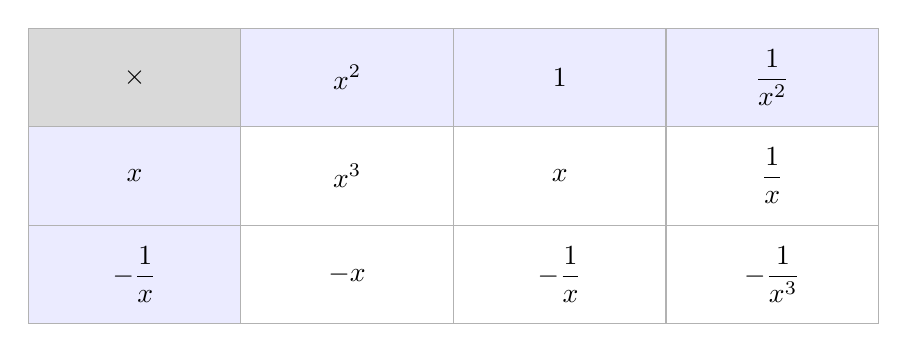
\begin{tikzpicture}[x=1cm,y=1cm]
\fill[gray!30] (0,0) rectangle (2.7,-1.25);
\draw[gray!60] (0,0) rectangle (2.7,-1.25);
\node at (1.35,-0.625) {$\displaystyle \times$};
\fill[blue!8] (2.7,0) rectangle (5.4,-1.25);
\draw[gray!60] (2.7,0) rectangle (5.4,-1.25);
\node at (4.05,-0.625) {$\displaystyle x^2$};
\fill[blue!8] (5.4,0) rectangle (8.1,-1.25);
\draw[gray!60] (5.4,0) rectangle (8.1,-1.25);
\node at (6.75,-0.625) {$\displaystyle 1$};
\fill[blue!8] (8.1,0) rectangle (10.8,-1.25);
\draw[gray!60] (8.1,0) rectangle (10.8,-1.25);
\node at (9.45,-0.625) {$\displaystyle \frac{1}{x^2}$};
\fill[blue!8] (0,-1.25) rectangle (2.7,-2.5);
\draw[gray!60] (0,-1.25) rectangle (2.7,-2.5);
\node at (1.35,-1.875) {$\displaystyle x$};
\fill[white] (2.7,-1.25) rectangle (5.4,-2.5);
\draw[gray!60] (2.7,-1.25) rectangle (5.4,-2.5);
\node at (4.05,-1.875) {$\displaystyle x^3$};
\fill[white] (5.4,-1.25) rectangle (8.1,-2.5);
\draw[gray!60] (5.4,-1.25) rectangle (8.1,-2.5);
\node at (6.75,-1.875) {$\displaystyle x$};
\fill[white] (8.1,-1.25) rectangle (10.8,-2.5);
\draw[gray!60] (8.1,-1.25) rectangle (10.8,-2.5);
\node at (9.45,-1.875) {$\displaystyle \frac{1}{x}$};
\fill[blue!8] (0,-2.5) rectangle (2.7,-3.75);
\draw[gray!60] (0,-2.5) rectangle (2.7,-3.75);
\node at (1.35,-3.125) {$\displaystyle -\frac{1}{x}$};
\fill[white] (2.7,-2.5) rectangle (5.4,-3.75);
\draw[gray!60] (2.7,-2.5) rectangle (5.4,-3.75);
\node at (4.05,-3.125) {$\displaystyle -x$};
\fill[white] (5.4,-2.5) rectangle (8.1,-3.75);
\draw[gray!60] (5.4,-2.5) rectangle (8.1,-3.75);
\node at (6.75,-3.125) {$\displaystyle -\frac{1}{x}$};
\fill[white] (8.1,-2.5) rectangle (10.8,-3.75);
\draw[gray!60] (8.1,-2.5) rectangle (10.8,-3.75);
\node at (9.45,-3.125) {$\displaystyle -\frac{1}{x^3}$};
\end{tikzpicture}
\end{center}
\small Grid for the first two brackets; the middle terms cancel to give $x^3-\tfrac{1}{x^3}$, which is then multiplied by the third bracket.\normalsize

\medskip\hrule

\section*{Expanding Brackets 36\quad\small\texttt{(a1-036)}}
\addcontentsline{toc}{section}{Expanding Brackets 36 (a1-036)}
\textit{Difficulty: Foundation \quad\textbar\quad Marks: 3}

\question{Expand and simplify \( \left(\frac{2}{y} - 3\right)\left(\frac{y}{2} + 1\right) \).}

\textbf{Worked solution.}

\textit{Expand the brackets}
\[\begin{gathered}
\begin{aligned} \left(\frac{2}{y} - 3\right)\left(\frac{y}{2} + 1\right) &= \frac{2}{y}\left(\frac{y}{2}+1\right) - 3\left(\frac{y}{2}+1\right) \\ &= \frac{2y}{2y} + \frac{2}{y} - \frac{3y}{2} - 3 \\ & = 1 +\frac{2}{y} - \frac{3y}{2} - 3 \\ & = \frac{2}{y} - \frac{3y}{2} - 2 \end{aligned}
\end{gathered}\]
Multiply the first, outer, inner, and last terms.

\begin{answerbox}
\textbf{Final answer:}\quad \(\displaystyle \frac{2}{y} - \frac{3y}{2} - 2\)
\end{answerbox}
\textbf{Area-model diagram.}

\begin{center}
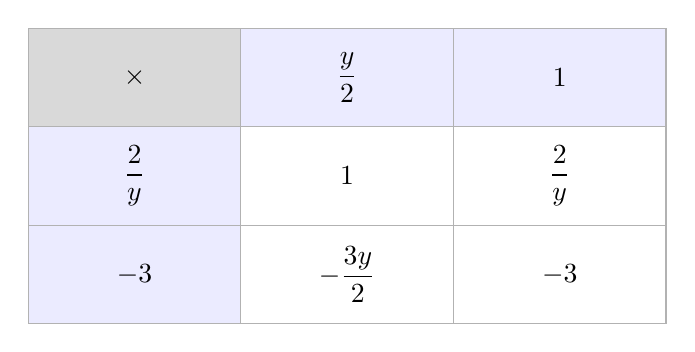
\begin{tikzpicture}[x=1cm,y=1cm]
\fill[gray!30] (0,0) rectangle (2.7,-1.25);
\draw[gray!60] (0,0) rectangle (2.7,-1.25);
\node at (1.35,-0.625) {$\displaystyle \times$};
\fill[blue!8] (2.7,0) rectangle (5.4,-1.25);
\draw[gray!60] (2.7,0) rectangle (5.4,-1.25);
\node at (4.05,-0.625) {$\displaystyle \frac{y}{2}$};
\fill[blue!8] (5.4,0) rectangle (8.1,-1.25);
\draw[gray!60] (5.4,0) rectangle (8.1,-1.25);
\node at (6.75,-0.625) {$\displaystyle 1$};
\fill[blue!8] (0,-1.25) rectangle (2.7,-2.5);
\draw[gray!60] (0,-1.25) rectangle (2.7,-2.5);
\node at (1.35,-1.875) {$\displaystyle \frac{2}{y}$};
\fill[white] (2.7,-1.25) rectangle (5.4,-2.5);
\draw[gray!60] (2.7,-1.25) rectangle (5.4,-2.5);
\node at (4.05,-1.875) {$\displaystyle 1$};
\fill[white] (5.4,-1.25) rectangle (8.1,-2.5);
\draw[gray!60] (5.4,-1.25) rectangle (8.1,-2.5);
\node at (6.75,-1.875) {$\displaystyle \frac{2}{y}$};
\fill[blue!8] (0,-2.5) rectangle (2.7,-3.75);
\draw[gray!60] (0,-2.5) rectangle (2.7,-3.75);
\node at (1.35,-3.125) {$\displaystyle -3$};
\fill[white] (2.7,-2.5) rectangle (5.4,-3.75);
\draw[gray!60] (2.7,-2.5) rectangle (5.4,-3.75);
\node at (4.05,-3.125) {$\displaystyle -\frac{3y}{2}$};
\fill[white] (5.4,-2.5) rectangle (8.1,-3.75);
\draw[gray!60] (5.4,-2.5) rectangle (8.1,-3.75);
\node at (6.75,-3.125) {$\displaystyle -3$};
\end{tikzpicture}
\end{center}
\medskip\hrule

\section*{Expanding Brackets 37\quad\small\texttt{(a1-037)}}
\addcontentsline{toc}{section}{Expanding Brackets 37 (a1-037)}
\textit{Difficulty: Foundation \quad\textbar\quad Marks: 3}

\question{Expand and simplify \( a^2b(a - b) + ab^2(a + b) \).}

\textbf{Worked solution.}

\textit{Expand both sets of brackets}
\[\begin{gathered}
\begin{aligned} a^2b(a - b) + ab^2(a + b) &= (a^3b - a^2b^2) + (a^2b^2 + ab^3) \\ &= a^3b - a^2b^2 + a^2b^2 + ab^3 \\ & = a^3b + ab^3 \end{aligned}
\end{gathered}\]
Multiply the terms outside by each term inside the brackets.

\begin{answerbox}
\textbf{Final answer:}\quad \(\displaystyle a^3b + ab^3\)
\end{answerbox}
\textbf{Area-model diagram.}

\begin{center}
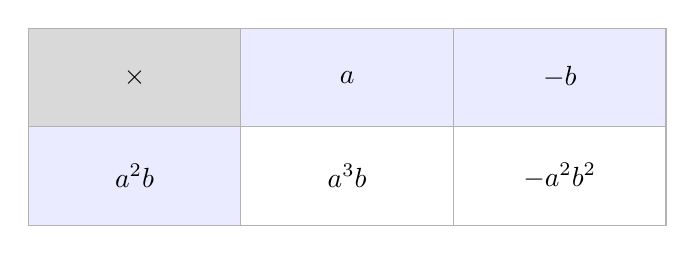
\begin{tikzpicture}[x=1cm,y=1cm]
\fill[gray!30] (0,0) rectangle (2.7,-1.25);
\draw[gray!60] (0,0) rectangle (2.7,-1.25);
\node at (1.35,-0.625) {$\displaystyle \times$};
\fill[blue!8] (2.7,0) rectangle (5.4,-1.25);
\draw[gray!60] (2.7,0) rectangle (5.4,-1.25);
\node at (4.05,-0.625) {$\displaystyle a$};
\fill[blue!8] (5.4,0) rectangle (8.1,-1.25);
\draw[gray!60] (5.4,0) rectangle (8.1,-1.25);
\node at (6.75,-0.625) {$\displaystyle -b$};
\fill[blue!8] (0,-1.25) rectangle (2.7,-2.5);
\draw[gray!60] (0,-1.25) rectangle (2.7,-2.5);
\node at (1.35,-1.875) {$\displaystyle a^2b$};
\fill[white] (2.7,-1.25) rectangle (5.4,-2.5);
\draw[gray!60] (2.7,-1.25) rectangle (5.4,-2.5);
\node at (4.05,-1.875) {$\displaystyle a^3b$};
\fill[white] (5.4,-1.25) rectangle (8.1,-2.5);
\draw[gray!60] (5.4,-1.25) rectangle (8.1,-2.5);
\node at (6.75,-1.875) {$\displaystyle -a^2b^2$};
\end{tikzpicture}
\end{center}
\small Grid for $a^2b(a-b)$; add the analogous grid for $ab^2(a+b)=a^2b^2+ab^3$.\normalsize

\medskip\hrule

\section*{Expanding Brackets 38\quad\small\texttt{(a1-038)}}
\addcontentsline{toc}{section}{Expanding Brackets 38 (a1-038)}
\textit{Difficulty: Foundation \quad\textbar\quad Marks: 2}

\question{Expand and simplify \( \left(2x + \frac{3}{x}\right)\left(2x - \frac{3}{x}\right) \).}

\textbf{Worked solution.}

\textit{Expand using the difference of two squares identity}
\[\begin{gathered}
\begin{aligned} \left(2x + \frac{3}{x}\right)\left(2x - \frac{3}{x}\right) & = 2x\left( 2x - \frac{3}{x}\right) + \frac{3}{x}\left( 2x - \frac{3}{x}\right) \\ & = 4x^2 - \frac{6x}{x} + \frac{6x}{x} - \frac{9}{x^2} \\ & = 4x^2 - 6 + 6 - \frac{9}{x^2} \\ & = 4x^2 - \frac{9}{x^2} \end{aligned}
\end{gathered}\]
Recognize the pattern \( (a+b)(a-b) = a^2 - b^2 \). Alternatively, expanding fully shows the middle terms cancel out: \( 4x^2 - \frac{6x}{x} + \frac{6x}{x} - \frac{9}{x^2} \).

\begin{answerbox}
\textbf{Final answer:}\quad \(\displaystyle 4x^2 - \frac{9}{x^2}\)
\end{answerbox}
\textbf{Area-model diagram.}

\begin{center}
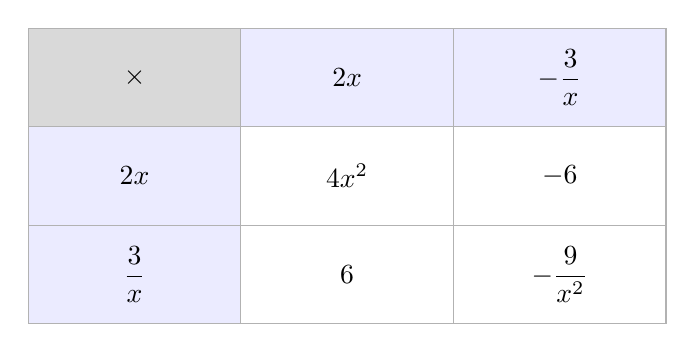
\begin{tikzpicture}[x=1cm,y=1cm]
\fill[gray!30] (0,0) rectangle (2.7,-1.25);
\draw[gray!60] (0,0) rectangle (2.7,-1.25);
\node at (1.35,-0.625) {$\displaystyle \times$};
\fill[blue!8] (2.7,0) rectangle (5.4,-1.25);
\draw[gray!60] (2.7,0) rectangle (5.4,-1.25);
\node at (4.05,-0.625) {$\displaystyle 2x$};
\fill[blue!8] (5.4,0) rectangle (8.1,-1.25);
\draw[gray!60] (5.4,0) rectangle (8.1,-1.25);
\node at (6.75,-0.625) {$\displaystyle -\frac{3}{x}$};
\fill[blue!8] (0,-1.25) rectangle (2.7,-2.5);
\draw[gray!60] (0,-1.25) rectangle (2.7,-2.5);
\node at (1.35,-1.875) {$\displaystyle 2x$};
\fill[white] (2.7,-1.25) rectangle (5.4,-2.5);
\draw[gray!60] (2.7,-1.25) rectangle (5.4,-2.5);
\node at (4.05,-1.875) {$\displaystyle 4x^2$};
\fill[white] (5.4,-1.25) rectangle (8.1,-2.5);
\draw[gray!60] (5.4,-1.25) rectangle (8.1,-2.5);
\node at (6.75,-1.875) {$\displaystyle -6$};
\fill[blue!8] (0,-2.5) rectangle (2.7,-3.75);
\draw[gray!60] (0,-2.5) rectangle (2.7,-3.75);
\node at (1.35,-3.125) {$\displaystyle \frac{3}{x}$};
\fill[white] (2.7,-2.5) rectangle (5.4,-3.75);
\draw[gray!60] (2.7,-2.5) rectangle (5.4,-3.75);
\node at (4.05,-3.125) {$\displaystyle 6$};
\fill[white] (5.4,-2.5) rectangle (8.1,-3.75);
\draw[gray!60] (5.4,-2.5) rectangle (8.1,-3.75);
\node at (6.75,-3.125) {$\displaystyle -\frac{9}{x^2}$};
\end{tikzpicture}
\end{center}
\small The off-diagonal terms $-6$ and $+6$ cancel: a difference of two squares.\normalsize

\medskip\hrule

\section*{Expanding Brackets 39\quad\small\texttt{(a1-039)}}
\addcontentsline{toc}{section}{Expanding Brackets 39 (a1-039)}
\textit{Difficulty: Foundation \quad\textbar\quad Marks: 3}

\question{Expand and simplify \( \left(x + \frac{2}{x}\right)^2 \).}

\textbf{Worked solution.}

\textit{Rewrite as two brackets and expand}
\[\begin{gathered}
\begin{aligned} \left(x + \frac{2}{x}\right)\left(x + \frac{2}{x}\right) &= x\left(x + \frac{2}{x}\right) + \frac{2}{x}\left(x + \frac{2}{x}\right) \\ &= x^2 + \frac{2x}{x} + \frac{2x}{x} + \frac{4}{x^2} = x^2 + 2 + 2 + \frac{4}{x^2} = x^2 + 4 + \frac{4}{x^2} \end{aligned}
\end{gathered}\]
Multiply every term in the first bracket by every term in the second bracket.

\begin{answerbox}
\textbf{Final answer:}\quad \(\displaystyle x^2 + 4 + \frac{4}{x^2}\)
\end{answerbox}
\textbf{Area-model diagram.}

\begin{center}
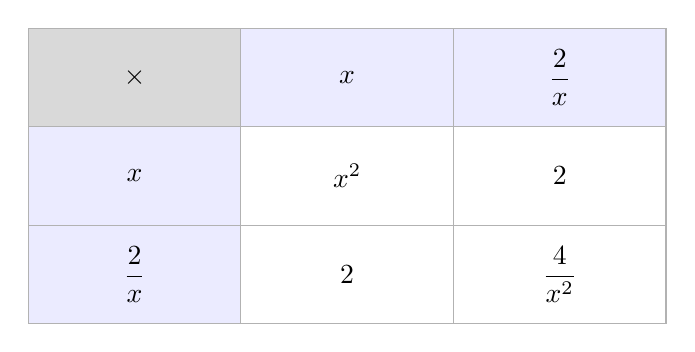
\begin{tikzpicture}[x=1cm,y=1cm]
\fill[gray!30] (0,0) rectangle (2.7,-1.25);
\draw[gray!60] (0,0) rectangle (2.7,-1.25);
\node at (1.35,-0.625) {$\displaystyle \times$};
\fill[blue!8] (2.7,0) rectangle (5.4,-1.25);
\draw[gray!60] (2.7,0) rectangle (5.4,-1.25);
\node at (4.05,-0.625) {$\displaystyle x$};
\fill[blue!8] (5.4,0) rectangle (8.1,-1.25);
\draw[gray!60] (5.4,0) rectangle (8.1,-1.25);
\node at (6.75,-0.625) {$\displaystyle \frac{2}{x}$};
\fill[blue!8] (0,-1.25) rectangle (2.7,-2.5);
\draw[gray!60] (0,-1.25) rectangle (2.7,-2.5);
\node at (1.35,-1.875) {$\displaystyle x$};
\fill[white] (2.7,-1.25) rectangle (5.4,-2.5);
\draw[gray!60] (2.7,-1.25) rectangle (5.4,-2.5);
\node at (4.05,-1.875) {$\displaystyle x^2$};
\fill[white] (5.4,-1.25) rectangle (8.1,-2.5);
\draw[gray!60] (5.4,-1.25) rectangle (8.1,-2.5);
\node at (6.75,-1.875) {$\displaystyle 2$};
\fill[blue!8] (0,-2.5) rectangle (2.7,-3.75);
\draw[gray!60] (0,-2.5) rectangle (2.7,-3.75);
\node at (1.35,-3.125) {$\displaystyle \frac{2}{x}$};
\fill[white] (2.7,-2.5) rectangle (5.4,-3.75);
\draw[gray!60] (2.7,-2.5) rectangle (5.4,-3.75);
\node at (4.05,-3.125) {$\displaystyle 2$};
\fill[white] (5.4,-2.5) rectangle (8.1,-3.75);
\draw[gray!60] (5.4,-2.5) rectangle (8.1,-3.75);
\node at (6.75,-3.125) {$\displaystyle \frac{4}{x^2}$};
\end{tikzpicture}
\end{center}
\small Grid for the perfect square $\left(x+\tfrac{2}{x}\right)^2$.\normalsize

\medskip\hrule

\section*{Expanding Brackets 40\quad\small\texttt{(a1-040)}}
\addcontentsline{toc}{section}{Expanding Brackets 40 (a1-040)}
\textit{Difficulty: Foundation \quad\textbar\quad Marks: 3}

\question{Expand and simplify \( \left(\frac{1}{x^2} - x\right)\left(x^3 - x\right) \).}

\textbf{Worked solution.}

\textit{Expand the brackets}
\[\begin{gathered}
\begin{aligned} \left(\frac{1}{x^2} - x\right)\left(x^3 - x\right) &= \frac{1}{x^2}\left( x^3 - x \right) - x(x^3-x) \\ & = \frac{x^3}{x^2}-\frac{x}{x^2} - x^4 + x^2\\ & = x-\frac{1}{x}-x^4+x^2  \end{aligned}
\end{gathered}\]
Distribute each term from the first bracket into the second bracket.

\begin{answerbox}
\textbf{Final answer:}\quad \(\displaystyle -x^4 + x^2 + x - \frac{1}{x}\)
\end{answerbox}
\textbf{Area-model diagram.}

\begin{center}
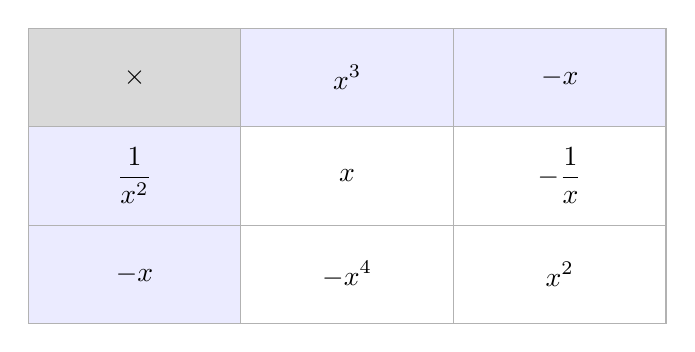
\begin{tikzpicture}[x=1cm,y=1cm]
\fill[gray!30] (0,0) rectangle (2.7,-1.25);
\draw[gray!60] (0,0) rectangle (2.7,-1.25);
\node at (1.35,-0.625) {$\displaystyle \times$};
\fill[blue!8] (2.7,0) rectangle (5.4,-1.25);
\draw[gray!60] (2.7,0) rectangle (5.4,-1.25);
\node at (4.05,-0.625) {$\displaystyle x^3$};
\fill[blue!8] (5.4,0) rectangle (8.1,-1.25);
\draw[gray!60] (5.4,0) rectangle (8.1,-1.25);
\node at (6.75,-0.625) {$\displaystyle -x$};
\fill[blue!8] (0,-1.25) rectangle (2.7,-2.5);
\draw[gray!60] (0,-1.25) rectangle (2.7,-2.5);
\node at (1.35,-1.875) {$\displaystyle \frac{1}{x^2}$};
\fill[white] (2.7,-1.25) rectangle (5.4,-2.5);
\draw[gray!60] (2.7,-1.25) rectangle (5.4,-2.5);
\node at (4.05,-1.875) {$\displaystyle x$};
\fill[white] (5.4,-1.25) rectangle (8.1,-2.5);
\draw[gray!60] (5.4,-1.25) rectangle (8.1,-2.5);
\node at (6.75,-1.875) {$\displaystyle -\frac{1}{x}$};
\fill[blue!8] (0,-2.5) rectangle (2.7,-3.75);
\draw[gray!60] (0,-2.5) rectangle (2.7,-3.75);
\node at (1.35,-3.125) {$\displaystyle -x$};
\fill[white] (2.7,-2.5) rectangle (5.4,-3.75);
\draw[gray!60] (2.7,-2.5) rectangle (5.4,-3.75);
\node at (4.05,-3.125) {$\displaystyle -x^4$};
\fill[white] (5.4,-2.5) rectangle (8.1,-3.75);
\draw[gray!60] (5.4,-2.5) rectangle (8.1,-3.75);
\node at (6.75,-3.125) {$\displaystyle x^2$};
\end{tikzpicture}
\end{center}
\medskip\hrule

\section*{Expanding Brackets 41\quad\small\texttt{(a1-041)}}
\addcontentsline{toc}{section}{Expanding Brackets 41 (a1-041)}
\textit{Difficulty: Foundation \quad\textbar\quad Marks: 4}

\question{Expand and simplify \( \left(p - \frac{1}{p}\right)\left(p + \frac{1}{p}\right)\left(p^2 + \frac{1}{p^2}\right) \).}

\textbf{Worked solution.}

\textit{Expand the first two brackets, then multiply by the third}
\[\begin{gathered}
\begin{aligned} &\left(p - \frac{1}{p}\right)\left(p + \frac{1}{p}\right)\left(p^2 + \frac{1}{p^2}\right) \\ &= \left[ p\left(p+\frac{1}{p}\right) - \frac{1}{p}\left(p+\frac{1}{p}\right) \right]\left(p^2 + \frac{1}{p^2}\right) \\ &= \left( p^2 - \frac{1}{p^2} \right)\left(p^2 + \frac{1}{p^2}\right) \\ &= p^2\left( p^2 + \frac{1}{p^2} \right) -\frac{1}{p^2}\left( p^2 +\frac{1}{p^2}\right) \\ &= p^4 + 1 - 1 - \frac{1}{p^4} \\ &= p^4 - \frac{1}{p^4} \end{aligned}
\end{gathered}\]
The first two brackets form a difference of two squares. The result multiplied by the third bracket forms another difference of two squares.

\begin{answerbox}
\textbf{Final answer:}\quad \(\displaystyle p^4 - \frac{1}{p^4}\)
\end{answerbox}
\textbf{Area-model diagram.}

\begin{center}
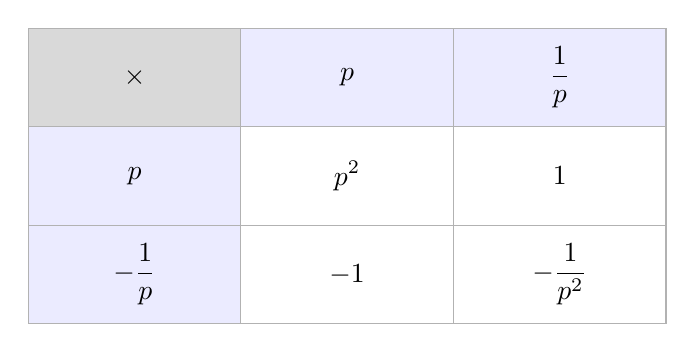
\begin{tikzpicture}[x=1cm,y=1cm]
\fill[gray!30] (0,0) rectangle (2.7,-1.25);
\draw[gray!60] (0,0) rectangle (2.7,-1.25);
\node at (1.35,-0.625) {$\displaystyle \times$};
\fill[blue!8] (2.7,0) rectangle (5.4,-1.25);
\draw[gray!60] (2.7,0) rectangle (5.4,-1.25);
\node at (4.05,-0.625) {$\displaystyle p$};
\fill[blue!8] (5.4,0) rectangle (8.1,-1.25);
\draw[gray!60] (5.4,0) rectangle (8.1,-1.25);
\node at (6.75,-0.625) {$\displaystyle \frac{1}{p}$};
\fill[blue!8] (0,-1.25) rectangle (2.7,-2.5);
\draw[gray!60] (0,-1.25) rectangle (2.7,-2.5);
\node at (1.35,-1.875) {$\displaystyle p$};
\fill[white] (2.7,-1.25) rectangle (5.4,-2.5);
\draw[gray!60] (2.7,-1.25) rectangle (5.4,-2.5);
\node at (4.05,-1.875) {$\displaystyle p^2$};
\fill[white] (5.4,-1.25) rectangle (8.1,-2.5);
\draw[gray!60] (5.4,-1.25) rectangle (8.1,-2.5);
\node at (6.75,-1.875) {$\displaystyle 1$};
\fill[blue!8] (0,-2.5) rectangle (2.7,-3.75);
\draw[gray!60] (0,-2.5) rectangle (2.7,-3.75);
\node at (1.35,-3.125) {$\displaystyle -\frac{1}{p}$};
\fill[white] (2.7,-2.5) rectangle (5.4,-3.75);
\draw[gray!60] (2.7,-2.5) rectangle (5.4,-3.75);
\node at (4.05,-3.125) {$\displaystyle -1$};
\fill[white] (5.4,-2.5) rectangle (8.1,-3.75);
\draw[gray!60] (5.4,-2.5) rectangle (8.1,-3.75);
\node at (6.75,-3.125) {$\displaystyle -\frac{1}{p^2}$};
\end{tikzpicture}
\end{center}
\small Grid for the first two brackets giving $p^2-\tfrac{1}{p^2}$; multiplying by $(p^2+\tfrac{1}{p^2})$ repeats the difference-of-squares pattern.\normalsize

\medskip\hrule

\section*{Expanding Brackets 42\quad\small\texttt{(a1-042)}}
\addcontentsline{toc}{section}{Expanding Brackets 42 (a1-042)}
\textit{Difficulty: Foundation \quad\textbar\quad Marks: 4}

\question{Expand and simplify \( p(p+q)-(p-q)(p+q) \).}

\textbf{Worked solution.}

\textit{Expand the first single bracket, and then expand the pair of brackets.}
\[\begin{gathered}
\begin{aligned}  p(p+q)-(p-q)(p+q) & = p^2+pq -p(p+q)+q(p+q) \\ & = p^2+pq - p^2-pq+pq+q^2 \\ &= q^2+pq \end{aligned}
\end{gathered}\]
Recognize the difference of two squares. The middle terms cancel out.

\begin{answerbox}
\textbf{Final answer:}\quad \(\displaystyle q^2+pq\)
\end{answerbox}
\textbf{Area-model diagram.}

\begin{center}
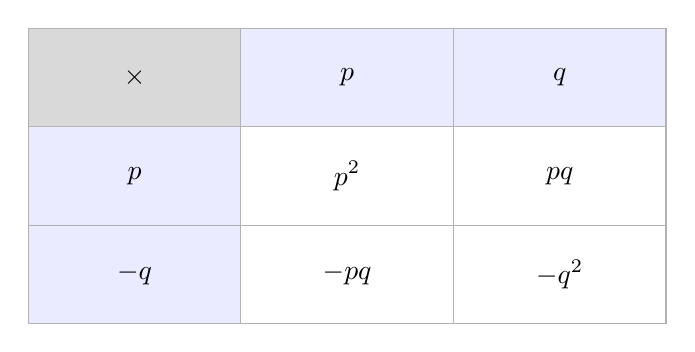
\begin{tikzpicture}[x=1cm,y=1cm]
\fill[gray!30] (0,0) rectangle (2.7,-1.25);
\draw[gray!60] (0,0) rectangle (2.7,-1.25);
\node at (1.35,-0.625) {$\displaystyle \times$};
\fill[blue!8] (2.7,0) rectangle (5.4,-1.25);
\draw[gray!60] (2.7,0) rectangle (5.4,-1.25);
\node at (4.05,-0.625) {$\displaystyle p$};
\fill[blue!8] (5.4,0) rectangle (8.1,-1.25);
\draw[gray!60] (5.4,0) rectangle (8.1,-1.25);
\node at (6.75,-0.625) {$\displaystyle q$};
\fill[blue!8] (0,-1.25) rectangle (2.7,-2.5);
\draw[gray!60] (0,-1.25) rectangle (2.7,-2.5);
\node at (1.35,-1.875) {$\displaystyle p$};
\fill[white] (2.7,-1.25) rectangle (5.4,-2.5);
\draw[gray!60] (2.7,-1.25) rectangle (5.4,-2.5);
\node at (4.05,-1.875) {$\displaystyle p^2$};
\fill[white] (5.4,-1.25) rectangle (8.1,-2.5);
\draw[gray!60] (5.4,-1.25) rectangle (8.1,-2.5);
\node at (6.75,-1.875) {$\displaystyle pq$};
\fill[blue!8] (0,-2.5) rectangle (2.7,-3.75);
\draw[gray!60] (0,-2.5) rectangle (2.7,-3.75);
\node at (1.35,-3.125) {$\displaystyle -q$};
\fill[white] (2.7,-2.5) rectangle (5.4,-3.75);
\draw[gray!60] (2.7,-2.5) rectangle (5.4,-3.75);
\node at (4.05,-3.125) {$\displaystyle -pq$};
\fill[white] (5.4,-2.5) rectangle (8.1,-3.75);
\draw[gray!60] (5.4,-2.5) rectangle (8.1,-3.75);
\node at (6.75,-3.125) {$\displaystyle -q^2$};
\end{tikzpicture}
\end{center}
\small Grid for $(p-q)(p+q)=p^2-q^2$; this is subtracted from $p(p+q)=p^2+pq$.\normalsize

\medskip\hrule

\section*{Expanding Brackets 43\quad\small\texttt{(a1-043)}}
\addcontentsline{toc}{section}{Expanding Brackets 43 (a1-043)}
\textit{Difficulty: Foundation \quad\textbar\quad Marks: 4}

\question{Expand and simplify \( (x+y)^3 \).}

\textbf{Worked solution.}

\textit{Expand the first two brackets, and then expand the final bracket.}
\[\begin{gathered}
\begin{aligned} (x+y)^3 = (x+y)(x+y)(x+y) & = \Big( (x+y)(x+y) \Big) (x+y) \\ & = \Big( x(x+y)+y(x+y) \Big)(x+y) \\ & = \Big( x^2+xy+xy+y^2 \Big)(x+y) \\ & = \Big( x^2+2xy+y^2 \Big)(x+y) \\ & = x(x^2+2xy+y^2)+y(x^2+2xy+y^2) \\ & = x^3+2x^2y+xy^2+x^2y+2xy^2+y^3 \\ & = x^3+3x^2y+3xy^2+y^3 \end{aligned}
\end{gathered}\]
Recognize the difference of two squares. The middle terms cancel out.

\begin{answerbox}
\textbf{Final answer:}\quad \(\displaystyle x^3+3x^2y+3xy^2+y^3\)
\end{answerbox}
\textbf{Area-model diagram.}

\begin{center}
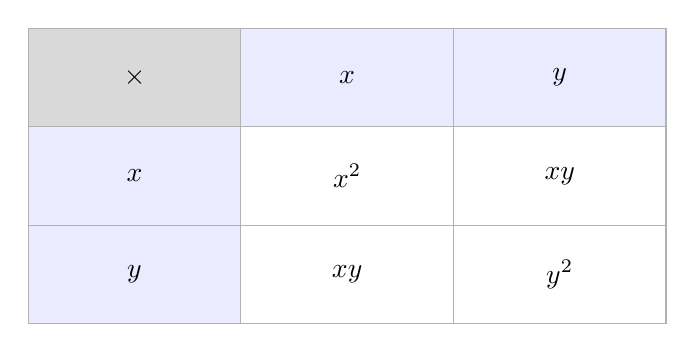
\begin{tikzpicture}[x=1cm,y=1cm]
\fill[gray!30] (0,0) rectangle (2.7,-1.25);
\draw[gray!60] (0,0) rectangle (2.7,-1.25);
\node at (1.35,-0.625) {$\displaystyle \times$};
\fill[blue!8] (2.7,0) rectangle (5.4,-1.25);
\draw[gray!60] (2.7,0) rectangle (5.4,-1.25);
\node at (4.05,-0.625) {$\displaystyle x$};
\fill[blue!8] (5.4,0) rectangle (8.1,-1.25);
\draw[gray!60] (5.4,0) rectangle (8.1,-1.25);
\node at (6.75,-0.625) {$\displaystyle y$};
\fill[blue!8] (0,-1.25) rectangle (2.7,-2.5);
\draw[gray!60] (0,-1.25) rectangle (2.7,-2.5);
\node at (1.35,-1.875) {$\displaystyle x$};
\fill[white] (2.7,-1.25) rectangle (5.4,-2.5);
\draw[gray!60] (2.7,-1.25) rectangle (5.4,-2.5);
\node at (4.05,-1.875) {$\displaystyle x^2$};
\fill[white] (5.4,-1.25) rectangle (8.1,-2.5);
\draw[gray!60] (5.4,-1.25) rectangle (8.1,-2.5);
\node at (6.75,-1.875) {$\displaystyle xy$};
\fill[blue!8] (0,-2.5) rectangle (2.7,-3.75);
\draw[gray!60] (0,-2.5) rectangle (2.7,-3.75);
\node at (1.35,-3.125) {$\displaystyle y$};
\fill[white] (2.7,-2.5) rectangle (5.4,-3.75);
\draw[gray!60] (2.7,-2.5) rectangle (5.4,-3.75);
\node at (4.05,-3.125) {$\displaystyle xy$};
\fill[white] (5.4,-2.5) rectangle (8.1,-3.75);
\draw[gray!60] (5.4,-2.5) rectangle (8.1,-3.75);
\node at (6.75,-3.125) {$\displaystyle y^2$};
\end{tikzpicture}
\end{center}
\small Grid for $(x+y)^2$; the result $x^2+2xy+y^2$ is then multiplied by $(x+y)$.\normalsize

\medskip\hrule

\section*{Expanding Brackets 44\quad\small\texttt{(a1-044)}}
\addcontentsline{toc}{section}{Expanding Brackets 44 (a1-044)}
\textit{Difficulty: Foundation \quad\textbar\quad Marks: 4}

\question{Expand and simplify \( (ab+cd)(ac-bd) \).}

\textbf{Worked solution.}

\textit{Expand the brackets}
\[\begin{gathered}
\begin{aligned} (ab+cd)(ac-bd) & = ab(ac-bd)+cd(ac-bd) \\ & = a^2bc-ab^2d+ac^2d-bcd^2 \end{aligned}
\end{gathered}\]
Multiply each term in the first bracket by each term in the second bracket.

\begin{answerbox}
\textbf{Final answer:}\quad \(\displaystyle a^2bc-ab^2d+ac^2d-bcd^2\)
\end{answerbox}
\textbf{Area-model diagram.}

\begin{center}
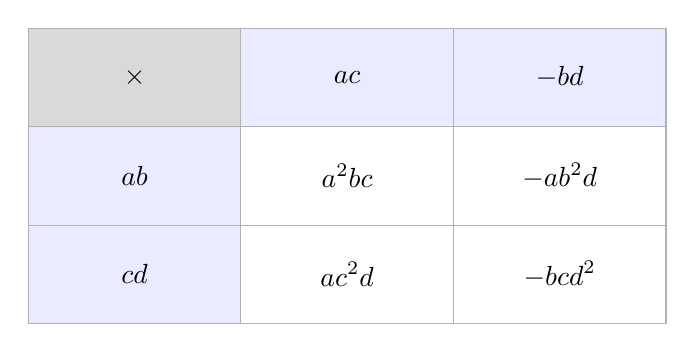
\begin{tikzpicture}[x=1cm,y=1cm]
\fill[gray!30] (0,0) rectangle (2.7,-1.25);
\draw[gray!60] (0,0) rectangle (2.7,-1.25);
\node at (1.35,-0.625) {$\displaystyle \times$};
\fill[blue!8] (2.7,0) rectangle (5.4,-1.25);
\draw[gray!60] (2.7,0) rectangle (5.4,-1.25);
\node at (4.05,-0.625) {$\displaystyle ac$};
\fill[blue!8] (5.4,0) rectangle (8.1,-1.25);
\draw[gray!60] (5.4,0) rectangle (8.1,-1.25);
\node at (6.75,-0.625) {$\displaystyle -bd$};
\fill[blue!8] (0,-1.25) rectangle (2.7,-2.5);
\draw[gray!60] (0,-1.25) rectangle (2.7,-2.5);
\node at (1.35,-1.875) {$\displaystyle ab$};
\fill[white] (2.7,-1.25) rectangle (5.4,-2.5);
\draw[gray!60] (2.7,-1.25) rectangle (5.4,-2.5);
\node at (4.05,-1.875) {$\displaystyle a^2bc$};
\fill[white] (5.4,-1.25) rectangle (8.1,-2.5);
\draw[gray!60] (5.4,-1.25) rectangle (8.1,-2.5);
\node at (6.75,-1.875) {$\displaystyle -ab^2d$};
\fill[blue!8] (0,-2.5) rectangle (2.7,-3.75);
\draw[gray!60] (0,-2.5) rectangle (2.7,-3.75);
\node at (1.35,-3.125) {$\displaystyle cd$};
\fill[white] (2.7,-2.5) rectangle (5.4,-3.75);
\draw[gray!60] (2.7,-2.5) rectangle (5.4,-3.75);
\node at (4.05,-3.125) {$\displaystyle ac^2d$};
\fill[white] (5.4,-2.5) rectangle (8.1,-3.75);
\draw[gray!60] (5.4,-2.5) rectangle (8.1,-3.75);
\node at (6.75,-3.125) {$\displaystyle -bcd^2$};
\end{tikzpicture}
\end{center}
\medskip\hrule

\section*{Expanding Brackets 45\quad\small\texttt{(a1-045)}}
\addcontentsline{toc}{section}{Expanding Brackets 45 (a1-045)}
\textit{Difficulty: Foundation \quad\textbar\quad Marks: 4}

\question{Expand and simplify \( (2x-1)^2(x+3) \).}

\textbf{Worked solution.}

\textit{Expand the brackets}
\[\begin{gathered}
\begin{aligned} (2x-1)^2(x+3) & = (2x-1)(2x-1)(x+3) \\ & = \Big( 2x(2x-1) -1(2x-1) \Big) (x+3) \\ & = \Big( 4x^2-2x-2x+1 \Big) (x+3) \\ & = \Big( 4x^2-4x+1 \Big) (x+3) \\ & = 4x^2(x+3)-4x(x+3)+1(x+3) \\ & = 4x^3+12x^2-4x^2-12x+x+3 \\ & = 4x^3+8x^2-11x+3 \end{aligned}
\end{gathered}\]
Multiply each term in the first bracket by each term in the second bracket.

\begin{answerbox}
\textbf{Final answer:}\quad \(\displaystyle 4x^3+8x^2-11x+3\)
\end{answerbox}
\textbf{Area-model diagram.}

\begin{center}
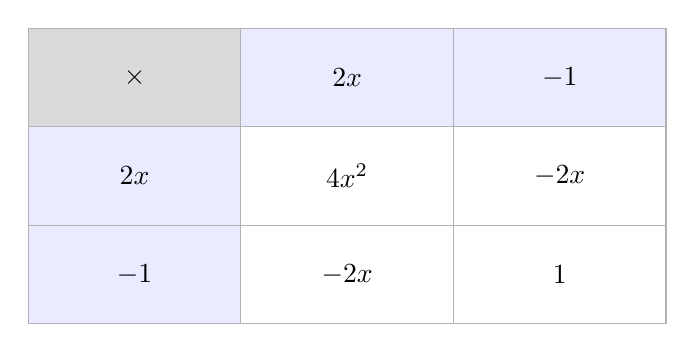
\begin{tikzpicture}[x=1cm,y=1cm]
\fill[gray!30] (0,0) rectangle (2.7,-1.25);
\draw[gray!60] (0,0) rectangle (2.7,-1.25);
\node at (1.35,-0.625) {$\displaystyle \times$};
\fill[blue!8] (2.7,0) rectangle (5.4,-1.25);
\draw[gray!60] (2.7,0) rectangle (5.4,-1.25);
\node at (4.05,-0.625) {$\displaystyle 2x$};
\fill[blue!8] (5.4,0) rectangle (8.1,-1.25);
\draw[gray!60] (5.4,0) rectangle (8.1,-1.25);
\node at (6.75,-0.625) {$\displaystyle -1$};
\fill[blue!8] (0,-1.25) rectangle (2.7,-2.5);
\draw[gray!60] (0,-1.25) rectangle (2.7,-2.5);
\node at (1.35,-1.875) {$\displaystyle 2x$};
\fill[white] (2.7,-1.25) rectangle (5.4,-2.5);
\draw[gray!60] (2.7,-1.25) rectangle (5.4,-2.5);
\node at (4.05,-1.875) {$\displaystyle 4x^2$};
\fill[white] (5.4,-1.25) rectangle (8.1,-2.5);
\draw[gray!60] (5.4,-1.25) rectangle (8.1,-2.5);
\node at (6.75,-1.875) {$\displaystyle -2x$};
\fill[blue!8] (0,-2.5) rectangle (2.7,-3.75);
\draw[gray!60] (0,-2.5) rectangle (2.7,-3.75);
\node at (1.35,-3.125) {$\displaystyle -1$};
\fill[white] (2.7,-2.5) rectangle (5.4,-3.75);
\draw[gray!60] (2.7,-2.5) rectangle (5.4,-3.75);
\node at (4.05,-3.125) {$\displaystyle -2x$};
\fill[white] (5.4,-2.5) rectangle (8.1,-3.75);
\draw[gray!60] (5.4,-2.5) rectangle (8.1,-3.75);
\node at (6.75,-3.125) {$\displaystyle 1$};
\end{tikzpicture}
\end{center}
\small Grid for $(2x-1)^2$; the result $4x^2-4x+1$ is then multiplied by $(x+3)$.\normalsize

\medskip\hrule

\end{document}
